\documentclass[10pt,openany]{book}\usepackage[]{graphicx}\usepackage[]{color}
%% maxwidth is the original width if it is less than linewidth
%% otherwise use linewidth (to make sure the graphics do not exceed the margin)
\makeatletter
\def\maxwidth{ %
  \ifdim\Gin@nat@width>\linewidth
    \linewidth
  \else
    \Gin@nat@width
  \fi
}
\makeatother

\definecolor{fgcolor}{rgb}{0.345, 0.345, 0.345}
\newcommand{\hlnum}[1]{\textcolor[rgb]{0.686,0.059,0.569}{#1}}%
\newcommand{\hlstr}[1]{\textcolor[rgb]{0.192,0.494,0.8}{#1}}%
\newcommand{\hlcom}[1]{\textcolor[rgb]{0.678,0.584,0.686}{\textit{#1}}}%
\newcommand{\hlopt}[1]{\textcolor[rgb]{0,0,0}{#1}}%
\newcommand{\hlstd}[1]{\textcolor[rgb]{0.345,0.345,0.345}{#1}}%
\newcommand{\hlkwa}[1]{\textcolor[rgb]{0.161,0.373,0.58}{\textbf{#1}}}%
\newcommand{\hlkwb}[1]{\textcolor[rgb]{0.69,0.353,0.396}{#1}}%
\newcommand{\hlkwc}[1]{\textcolor[rgb]{0.333,0.667,0.333}{#1}}%
\newcommand{\hlkwd}[1]{\textcolor[rgb]{0.737,0.353,0.396}{\textbf{#1}}}%
\let\hlipl\hlkwb

\usepackage{framed}
\makeatletter
\newenvironment{kframe}{%
 \def\at@end@of@kframe{}%
 \ifinner\ifhmode%
  \def\at@end@of@kframe{\end{minipage}}%
  \begin{minipage}{\columnwidth}%
 \fi\fi%
 \def\FrameCommand##1{\hskip\@totalleftmargin \hskip-\fboxsep
 \colorbox{shadecolor}{##1}\hskip-\fboxsep
     % There is no \\@totalrightmargin, so:
     \hskip-\linewidth \hskip-\@totalleftmargin \hskip\columnwidth}%
 \MakeFramed {\advance\hsize-\width
   \@totalleftmargin\z@ \linewidth\hsize
   \@setminipage}}%
 {\par\unskip\endMakeFramed%
 \at@end@of@kframe}
\makeatother

\definecolor{shadecolor}{rgb}{.97, .97, .97}
\definecolor{messagecolor}{rgb}{0, 0, 0}
\definecolor{warningcolor}{rgb}{1, 0, 1}
\definecolor{errorcolor}{rgb}{1, 0, 0}
\newenvironment{knitrout}{}{} % an empty environment to be redefined in TeX

\usepackage{alltt}



%\input{c:/aaaWork/zGnrlLatex/BookPreamble_HC}   % use for the hard-copy version
\input{c:/aaaWork/zGnrlLatex/BookPreamble}
\hypersetup{pdftitle = MTH107 Notes}
\input{c:/aaaWork/zGnrlLatex/JustRPreamble}
\usepackage{animate}
\usepackage{titlesec}
\titlespacing\section{0pt}{12pt plus 4pt minus 2pt}{0pt plus 2pt minus 2pt}
\titlespacing\subsection{-3pt}{12pt plus 4pt minus 2pt}{0pt plus 2pt minus 2pt}
\titlespacing\subsubsection{-3pt}{12pt plus 4pt minus 2pt}{0pt plus 2pt minus 2pt}
\renewcommand{\chaptername}{Module}
\IfFileExists{upquote.sty}{\usepackage{upquote}}{}
\begin{document}




  \frontmatter
    %MAKE MINI TABLE OF CONTENTS for each chapter ----------------------------------
\dominitoc
\setcounter{minitocdepth}{1} %sets the depth to show in chapter TOC -- 0 is chapters, 1 would be sections, etc.

\VerbatimFootnotes  % allows verbatim in footnotes

%TITLE PAGE --------------------------------------------------------------------
\begin{titlepage}
\begin{center}

% Upper part of the page
\textsc{\LARGE Northland College}\\[0.5cm]
\textsc{\Large MTH107 -- Statistical Analysis and Interpretation}\\[1.5cm]

\HRuleW \\
\HRule \\[1cm]
{ \huge \bfseries Introduction to Statistical Analysis and Interpretation}\\[1cm]
\HRule \\
\HRuleW \\[1.5cm]

% Author and supervisor
\begin{minipage}{0.4\textwidth}
\begin{flushleft}
%  \Large \emph{Author:}\\ Dr. Derek H. Ogle
  \Large \emph{Instructors:}\\Dr. Derek H. Ogle \\ Jodi Supanich
\end{flushleft}
\end{minipage}
\begin{minipage}{0.4\textwidth}
\begin{flushright} 
  \Large \emph{Department:} \\ Mathematical Sciences
%  \Large \emph{Department:} \\ Mathematical Sciences \\ Mathematical Sciences
\end{flushright}
\end{minipage}

\vfill

% Bottom of the page
%\includegraphics[width=4in]{Title.JPG} \\[2.5cm]
{\Large \today}

\end{center}

\end{titlepage}

%PREFACE -----------------------------------------------------------------------
\cleardoublepage                          %not sure why but is needed so that TOC entry will point to right start page
\phantomsection                           %not sure why but is needed so that TOC entry will point to right start page
\setlength{\cftbeforepartskip}{0.4em}     %set space before parts in TOC to smaller number for Preface
\addcontentsline{toc}{part}{Preface}      %put a preface item as a part into TOC
\vspace{-120pt}
\chapter*{Preface}                        %star means that the preface won't be numbered in TOC
\vspace{-80pt}
\section*{The ``Book''}
This document serves as the ``text'' for the MTH107 course taught by Derek Ogle at Northland College.  The use of this ``book'' as the class ``text'' stems from three primary concerns I had about teaching from a third-party textbook.  First, it seems that every textbook available covered more chapters of material than I could cover in a one semester course.  I was uncomfortable asking you (the student) to buy a textbook that was not used completely.  Second, it seemed to me that textbook authors often write for professors rather than students.  This leads to an extreme amount of detail in texts that does not fall within the learner outcomes or objectives that I have identified for this class.  In other words, you were left with the ``trick'' of having to identify exactly what I thought was important in each chapter.  This exercise, in my opinion, detracts from time and effort that should be spent learning the material that is important.  Third, it seems that my teaching style and some of my language differed from each and every textbook.  This created the situation of having to explain when and where to substitute my language into the textbook, which created a level of confusion that was not necessary.  In addition, this created the uncomfortable situation, for both you and me, of feeling that assessments that were written by me differed in orientation from the problems or exercises written by the third-party author.  With these concerns in mind, this ``book'' provides a ``text'' for students in MTH107 that (1) contains only the chapters of material that I will cover during the course of the semester, (2) contains only material that matches the intended learning outcomes for the course, and (3) is written in my style with my language and emphases.

One note to bear in mind as you interact with this ``book'' is that it has been distilled to the barest amount of material that I feel is required to meet the learning outcomes for this course.  Thus, none of the material should be skipped.  In addition, all exercises and problems have been written by me (though some data are from other texts) and, thus, reflect the type of questions that I am likely to ask and the activities that I feel will lead to learning.  Thus, you should carefully study the examples and work all of the review exercises and homework problems provided.

This ``book'' is distributed in electronic PDF format and can be viewed with the free Adobe Acrobat Reader software\footnote{Available for free download at \href{http://www.adobe.com/products/acrobat/readermain.html}{www.adobe.com/products/acrobat/readermain.html}.}.  The electronic version of this ``book'' has the following characteristics.

\begin{Itemize}
  \item Internal links exist to figures, tables, equations, chapters, sections, footnotes, and appendices.  All internal links appear as red text in the document.  You can return to where you were by right-clicking on the page and selecting ``previous view`` or simultaneously pressing the ``ALT'' key and the left arrow key.  Example links are as follows: to \figref{fig:VarTypes}, to \tabrefp{tab:KreherParkPbconc}, to \chapref{chap:Foundations}, and to equation \eqref{eqn:SampleMean}.
  \item External links exist to data files and third-party web pages with additional information and will appear as fuchsia text (e.g., to the \href{https://sites.google.com/site/ncstats/data/LakeSuperiorIce.txt}{LakeSuperiorIce.txt} data file).  These items can only be accessed if you are connected to the internet.
  \item Chapters of the text can be accessed by the table of contents that appears on the left-side of the PDF document.  In addition, a table of contents for items within a chapter is found on the first page of each chapter.
\end{Itemize}

Finally, please report all questions, problems, corrections, or concerns about these notes directly to me at \href{mailto:dogle@northland.edu}{dogle@northland.edu}.


\section*{R Statistical Software}
The R statistical programming language R is used throughout this text to construct graphics, perform statistical calculations, and test hypotheses.  R is a command-line driven ``language'' where calculations and graph construction is performed by typing commands rather than selecting menu items and options in dialog boxes.  While this form of interaction with a computer may initially seem like a drawback to using R, I have chosen to use R in this class for several strong reasons.  It is my experience that this very powerful language is becoming increasingly popular among applied researchers in a wide variety of fields.  R has several advantages that contribute to this surge in popularity:

\begin{Itemize}
  \item R is free, open source, and runs on Windows, Macintosh, and Unix/Linux platforms;
  \item The programming language in R is very powerful, flexible, and has many built-in statistical functions;
  \item The programming language is easy to learn for basic analyses;
  \item R has excellent graphing capabilities that are extensible;
  \item The programming language is easily extended with user-written functions;
  \item Further developments of the programming language are continuous and made available by a large group of international researchers; and
  \item The next step to programming other languages will be made easier by a student's experience with the R programming language.
\end{Itemize}

I know of no other free computer package that can be used in the variety of ways that R can be used in applied research.  Thus, even though R has a rather steep learning curve, I feel that the benefits of this program make it useful as the primary analytic tool for the methods learned in this course (and beyond).

Specific aspects of R are introduced and integrated throughout this ``book.''  It should be noted that the complete capabilities of R will not be addressed in this ``book.''  Rather the specific commands required to complete the analyses of this course will be described.  A thorough introduction to R is available as a PDF file with the downloaded program.  In addition, very good introductions to R for basic statistics are found in widely available resources \footnote{The interested reader is referred to \textsc{Introductory Statistics with R} (Dalgaard, P. 2002.) and \textsc{Using R for Introductory Statistics} (Verzani, J. 2004).  Previous versions of the latter are available on the web by searching for \verb+"SimpleR"+.  The Dalgaard volume is available in our library.}.

Directions for installing R, RStudio, and packages for R are described in \sectref{sect:RSetup}.

\section*{Acknowledgments}
I have used various incarnations of this ``book'' since Fall 2001.  Watching students interact with the material presented here has helped form my ideas for how best to present this information.  I thank all of these students for their patience with me in this endeavor with a very special thanks to those students that took the time to nicely tell me where there were mistakes, points of confusion, or areas that lacked clarity.  I hope that you, as you use this book, will do the same \footnote{You can contact me at \href{mailto:dogle@northland.edu}{dogle@northland.edu}.} as this is incredibly helpful to any author.

I also am deeply thankful to my colleague at Northland College, Dr. Susan (Annette) Nelson, as she identified many grammatical and editorial problems with the ``book'' in Summer 2011 that motivated me to make considerable improvements in the tone, language, and look of the ``book.''  She noticed things that my eyes just would not see and I am very thankful to her for that.

Of course, I don't have the luxury of just giving ideas and having someone else write for me so any errors, inconsistencies, lack of clarity, or conceptual failings are mine and mine alone.


%TABLE OF CONTENTS ---------------------------------------------------------------------------------------------------
\setcounter{tocdepth}{0} %sets the depth to show in TOC -- 0 is chapters, 1 would be sections, etc.

%modify what the parts look like
\renewcommand{\cftpartfont}{\scshape}                          %changes to small caps

%modify what the chapters look like
\setlength{\cftchapindent}{1.5em}                              %indent the chapters
\setlength{\cftbeforechapskip}{0.4em}                          %set the space between chapters -- reduce to 0.2 if depth is set to 0

%modify what the sections look like
\setlength{\cftsecindent}{3.8em}                               %indent the sections --- doesn't seem to work
\setlength{\cftbeforesecskip}{0.2em}                           %set the space between sections

\newpage                                                       %need this so that the TOC will start on its own page
\tableofcontents                                               %build the table of contents

%SETTING FOR LEAVING FRONT MATTER AND GOING TO MAIN DOCUMENT ---------------------------------------------------------
\addtocontents{toc}{\setlength{\cftbeforepartskip}{1.5em}}     %increase distance before parts in the main TOC
\addtocontents{toc}{\cftpagenumbersoff{part}}                  %so page numbers won't appear for parts in the main TOC 

  \mainmatter
    \part{Beginnings}



\chapter{Why Statistics is Important} \label{chap:WhyStatsImportant}
\begin{ChapObj}{\boxwidth}
  \textbf{Objectives:}
  \begin{Enumerate}
    \item Describe the two major reasons why statistics is important for understanding populations.
    \item Define natural and sampling variability.
    \item Describe ``difficulties'' in making conclusions about population caused by sampling variability.
    \item Define ``statistics'' (as a field of study).
    \item Appreciate the importance of statistics in scientific inquiry.
  \end{Enumerate}
\end{ChapObj}

\minitoc
\newpage

\section{Realities}\label{sect:Realities}
\lettrine{T}{he city of Ashland} performed an investigation in the area of Kreher Park \figrefp{fig:KreherParkMap} when considering the possible expansion of an existing wastewater treatment facility in 1989. The discovery of contamination from creosote waste in the subsoils and ground water at Kreher Park prompted the city to abandon the project. A subsequent assessment by the Wisconsin Department of Natural Resources (WDNR) indicated elevated levels of hazardous substances in soil borings, ground water samples, and in the sediments of Chequamegon Bay directly offshore of Kreher Park. In 1995 and 1999, the Northern States Power Company conducted investigations that further defined the area of contamination and confirmed the presence of specific contaminants associated with coal tar wastes. This site is now listed as a superfund site and is being given considerably more attention.\footnote{More information at the \href{https://cumulis.epa.gov/supercpad/cursites/csitinfo.cfm?id=0507952}{EPA} and the \href{http://dnr.wi.gov/topic/brownfields/ashland.html}{WDNR} websites.}

\begin{figure}[htbp]
  \centering
    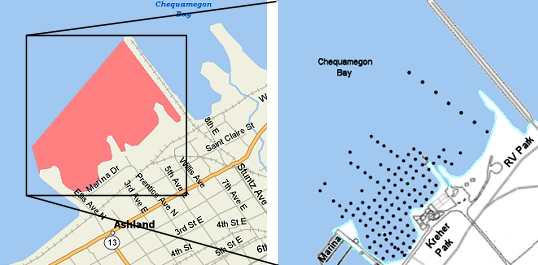
\includegraphics[width=6in]{Figs/Kreher_Park_Map.png}
  \caption{Location of the Ashland superfund site (left) with the location of 119 historical sediment sampling sites (right).}
  \label{fig:KreherParkMap}
\end{figure}

The WDNR wants to study elements in the sediment (among other things) in the entire 3000 m$^2$ area shaded in \figref{fig:KreherParkMap}. Is it physically possible to examine every square meter of that area?  Is it prudent, ecologically and economically, to examine every square meter of this area?  The answer, of course, is ``no.''  How then will the WDNR be able to make conclusions about this entire area if they cannot reasonably examine the whole area?  The most reasonable solution is to sample a subset of the area and use the results from this sample to make inferences about the entire area.

Methods for properly selecting a sample that fairly represents a larger collection of individuals are an important area of study in statistics. For example, the WDNR would not want to sample areas that are only conveniently near shore because this will likely not be an accurate representation of the entire area. In this example, it appears that the WDNR used a grid to assure a relatively even dispersal of samples throughout the study area \figrefp{fig:KreherParkMap}. Methods for choosing the number of individuals to select and how to select those individuals are discussed in \modref{chap:DataProd}.


Suppose that the WDNR measured the concentration of lead at each of the 119 locations shown in \figref{fig:KreherParkMap}. Further suppose that they presented their results at a public meeting by simply showing the list of lead concentration measurements \tabrefp{tab:KreherParkPbconc}.\footnote{These are hypothetical data for this site.}  Is it easy to make conclusions about what these data mean from this type of presentation?

\begin{table}[htbp]   \label{tab:KreherParkPbconc}
  \caption{Lead concentration ($\mu g \cdot m^{-3}$) from 119 sites in Kreher Park superfund site.}
  \begin{center}
% latex table generated in R 3.4.0 by xtable 1.8-2 package
% Sun May 21 17:06:38 2017
\begin{tabular}{rrrrrrrrrrrrrrr}
  \hline
  \hline
0.91 & 1.09 & 1.00 & 1.09 & 1.06 & 0.98 & 0.98 & 0.94 & 0.89 & 1.09 & 0.91 & 1.06 & 0.81 & 0.90 & 1.21 \\ 
  1.03 & 0.95 & 1.14 & 0.99 & 0.99 & 0.96 & 1.13 & 0.84 & 1.03 & 0.86 & 0.98 & 1.04 & 0.91 & 1.27 & 0.90 \\ 
  0.87 & 1.23 & 1.12 & 0.98 & 0.79 & 1.10 & 1.06 & 1.09 & 0.73 & 0.81 & 1.18 & 0.92 & 0.82 & 1.11 & 0.97 \\ 
  1.24 & 1.06 & 1.09 & 0.78 & 0.94 & 1.08 & 0.91 & 0.98 & 1.22 & 1.04 & 0.77 & 1.18 & 0.93 & 1.14 & 0.94 \\ 
  1.05 & 0.91 & 1.14 & 0.93 & 0.94 & 0.90 & 1.05 & 1.36 & 1.02 & 0.93 & 1.09 & 1.17 & 0.91 & 1.06 & 0.95 \\ 
  0.88 & 0.67 & 1.12 & 1.06 & 0.99 & 0.89 & 0.83 & 0.99 & 1.33 & 1.00 & 1.05 & 1.11 & 1.01 & 1.25 & 0.96 \\ 
  1.07 & 1.17 & 1.01 & 1.20 & 1.17 & 1.05 & 1.21 & 1.10 & 1.07 & 1.01 & 1.16 & 1.24 & 0.86 & 0.90 & 1.07 \\ 
  1.11 & 0.99 & 0.70 & 0.98 & 1.11 & 1.12 & 1.30 & 1.00 & 0.89 & 0.91 & 0.95 & 1.08 & 1.02 & 0.93 &  \\ 
   \hline
\end{tabular}

  \end{center}
\end{table}

Instead, suppose that the scientists brought a simple plot of the frequency of observed lead concentrations and brief numerical summaries \figrefp{fig:KreherParkPbhist} to the meeting. With these one can easily see that the measurements were fairly symmetric with no obviously ``weird'' values. The lead concentrations ranged from as low as 0.67 $\mu g \cdot m^{-3}$ to as high as 1.36 $\mu g \cdot m^{-3}$ with the measurements centered on approximately 1.0 $\mu g \cdot m^{-3}$. These summaries are discussed in detail in \modref{chap:UnivEDAQuant}. However, at this point, note that summarizing large quantities of data with few graphical or numerical summaries makes it is easier to identify meaning from the data.

\begin{knitrout}
\definecolor{shadecolor}{rgb}{0.922, 0.922, 0.922}\color{fgcolor}\begin{figure}[hbtp]

{\centering 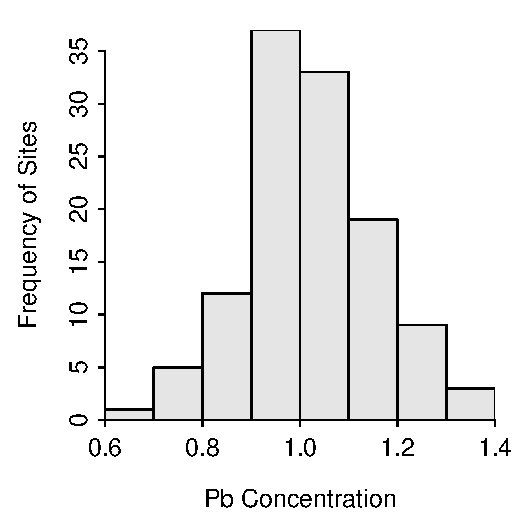
\includegraphics[width=.4\linewidth]{Figs/KreherParkPbhist-1} 
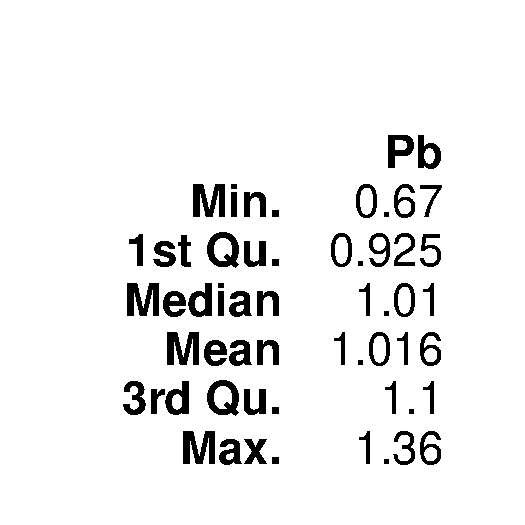
\includegraphics[width=.4\linewidth]{Figs/KreherParkPbhist-2} 

}

\caption[Histogram and summary statistics of lead concentration measurements ($\mu g \cdot m^{-3}$) at each of 119 sites in Kreher Park superfund site]{Histogram and summary statistics of lead concentration measurements ($\mu g \cdot m^{-3}$) at each of 119 sites in Kreher Park superfund site.}\label{fig:KreherParkPbhist}
\end{figure}


\end{knitrout}

A critical question at this point is whether or not the results from the one sample of 119 sites perfectly represents the results for the entire area. One way to consider this question is to examine the results obtained from another sample of 119 sites. The results from this second sample \figrefp{fig:KreherParkPbhist1} are clearly, though not radically, different from the results of the first sample. Thus, it is seen that any one sample from a larger whole will not perfectly represent the large whole. This will lead to some uncertainty in our summaries of the larger whole.

\begin{knitrout}
\definecolor{shadecolor}{rgb}{0.922, 0.922, 0.922}\color{fgcolor}\begin{figure}[hbtp]

{\centering 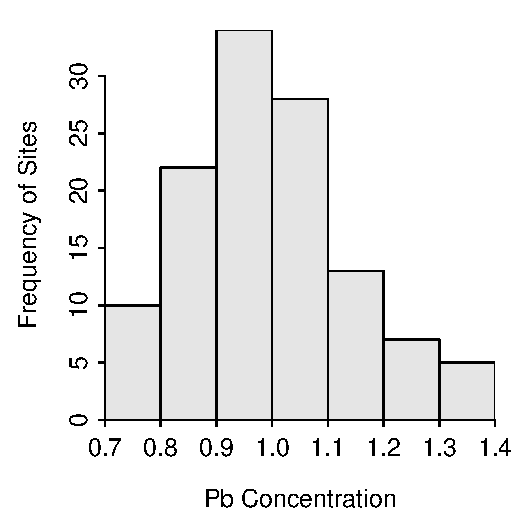
\includegraphics[width=.4\linewidth]{Figs/KreherParkPbhist1-1} 
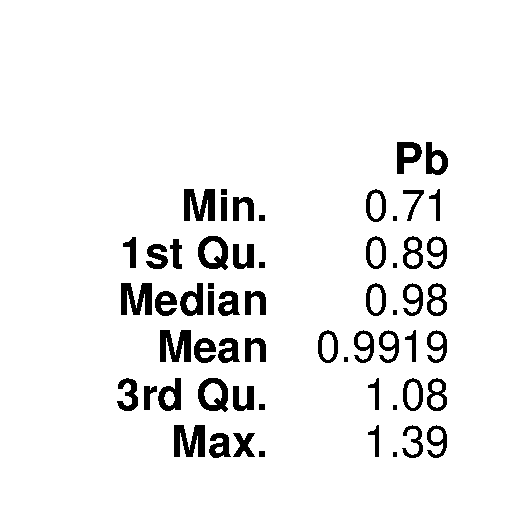
\includegraphics[width=.4\linewidth]{Figs/KreherParkPbhist1-2} 

}

\caption[Kreher Park 1]{Histogram and summary statistics of lead concentration measurements ($\mu g \cdot m^{-3}$) at each of 119 sites (different from the sites shown in \figref{fig:KreherParkPbhist}) in Kreher Park superfund site.}\label{fig:KreherParkPbhist1}
\end{figure}


\end{knitrout}

\vspace{18pt}
The results from two different samples do not perfectly agree because each sample contains different individuals (sites in this example), and no two individuals are exactly alike. The fact that no two individuals are exactly alike is \textbf{natural variability}\index{Natural Variability!Definition}, because of the ``natural'' differences that occur among individuals. The fact that the results from different samples are different is called \textbf{sampling variability}\index{Sampling Variability!Definition}. If there was no natural variability, then there would be no sampling variability. If there was no sampling variability, then the field of statistics would not be needed because a sample (even of one individual) would perfectly represent the larger group of individuals. Thus, understanding variability is at the core of statistical practice. Natural and sampling variability will be revisited continuously throughout this course.

This may be unsettling! First, it was shown that an entire area or all of the individuals of interest cannot be examined. It was then shown that a sample of individuals from the larger whole did not perfectly represent the larger whole. Furthermore, each sample is unique and will likely lead to a (slightly) different conclusion. These are all real and difficult issues faced by the practicing scientist and considered by the informed consumer. However, the field of statistics is designed to ``deal with'' these issues such that the results from a relatively small subset of measurements can be used to make conclusions about the entire collection of measurements.

\warn{Statistics provides methods for overcoming the difficulties caused by the requirement of sampling and the presence of sampling variability.}


\section{Major Goals or Purposes of Statistics}
As seen in the Kreher Park example, the field of statistics has two primary purposes. First, statistics provides methods to summarize large quantities of data into concise and informative numerical or graphical summaries. For example, it was easier to discern the general underlying structure of the lead measurements from the statistics and histograms presented in Figures \ref{fig:KreherParkPbhist} and \ref{fig:KreherParkPbhist1}, than it was from the full list of lead measurements in \tabref{tab:KreherParkPbconc}. Second, statistical methods allow inferences to be made about all individuals (i.e., a population) from a few individuals (i.e., a sample).\footnote{Population and sample are defined more completely in \sectref{sect:IVPPSS}.}


\section{Definition of Statistics}
Statistics is the science of collecting, organizing, and interpreting numerical information or data \citep{MooreMcCabe1998}\index{Statistics, Field of!Definition}. People study statistics for a variety of reasons, including \citep{Bluman2000}:
\begin{Enumerate}
  \item To understand the statistical studies performed in their field (i.e., be knowledgeable about the vocabulary, symbols, concepts, and statistical procedures used in those studies).
  \item To conduct research in their field (i.e., be able to design experiments and samples; collect, organize, analyze, and summarize data; make reliable predictions or forecasts for future use; and communicate statistical results).
  \item To be better consumers of statistical information.
\end{Enumerate}

Statistics permeates a wide variety of disciplines. \cite{MooreMcCabe1998} state:
\begin{quote}
The study and collection of data are important in the work of many professions, so that training in the science of statistics is valuable preparation for a variety of careers. Each month, for example, government statistical offices release the latest numerical information on unemployment and inflation. Economists and financial advisers, as well as policy makers in government and business study these data in order to make informed decisions. Doctors must understand the origin and trustworthiness of the data that appear in medical journals if they are to offer their patients the most effective treatments. Politicians rely on data from polls of public opinion. Business decisions are based on market research data that reveal customer tastes. Farmers study data from field trials of new crop varieties. Engineers gather data on the quality and reliability of manufactured products. Most areas of academic study make use of numbers, and therefore also make use of the methods of statistics.
\end{quote}



\chapter{Foundational Definitions} \label{chap:FoundationalDefinitions}
\begin{ChapObj}{\boxwidth}
  \textbf{Objectives:}
  \begin{Enumerate}
    \item Describe what an individual is.
    \item Describe what a population and a sample are and how they differ.
    \item Describe what a parameter and a statistic are and how they differ.
    \item Describe how a population, parameter, sample, and statistic are related.
    \item Identify the individual, variable(s), population, parameter(s), sample, and statistic(s) (IVPPSS) in a given situation.
    \item Identify variable types in context.
  \end{Enumerate}
\end{ChapObj}

\minitoc
\newpage

\lettrine{S}{tatistical inference is the process} of forming conclusions about a parameter of a population from statistics computed from individuals in a sample.\index{Inference!Definition}\footnote{Formal methods of inference are discussed beginning with \modref{chap:ProbIntro}.} Thus, understanding statistical inference requires understanding the difference between a population and a sample and a parameter and a statistic. And, to properly describe those items, the individual and variable(s) of interest must be identified. Understanding and identifying these six items is the focus of this module.

The following hypothetical example is used throughout this module. Assume that we are interested in the average length of 1015 fish in Square Lake. To illustrate important concepts in this module, assume that all information for all 1015 fish in this lake is known \figrefp{fig:SquareLakePopn}. In ``real life'' this complete information would not be known.

\begin{knitrout}
\definecolor{shadecolor}{rgb}{0.922, 0.922, 0.922}\color{fgcolor}\begin{figure}[hbtp]

{\centering 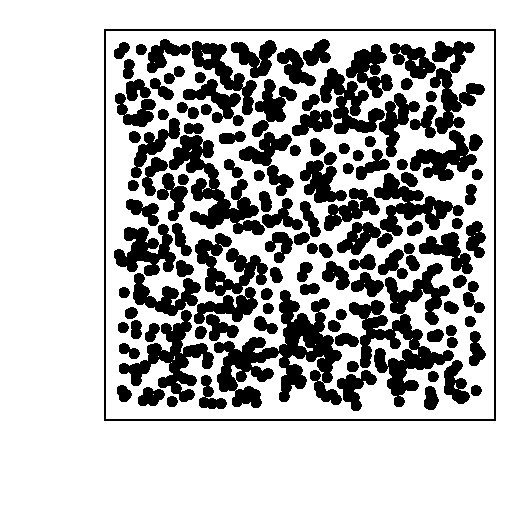
\includegraphics[width=.4\linewidth]{Figs/SquareLakePopn-1} 
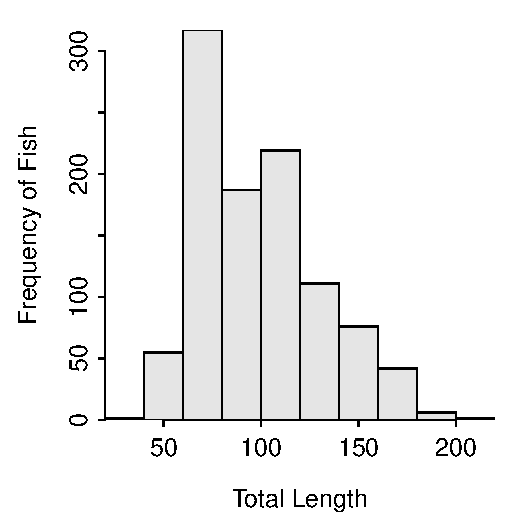
\includegraphics[width=.4\linewidth]{Figs/SquareLakePopn-2} 

}

\caption[Schematic representation of individual fish (i.e., dots]{Schematic representation of individual fish (i.e., dots; \textbf{Left}) and histogram (\textbf{Right}) of the total length of the 1015 fish in Square Lake.}\label{fig:SquareLakePopn}
\end{figure}


\end{knitrout}

\section{Definitions} \label{sect:IVPPSS}
The \textbf{individual} in a statistical analysis is one of the ``items'' examined by the researcher.\index{Individual, Definition}  Sometimes the individual is a person, but it may be an animal, a piece of wood, a location, a particular time, or an event. It is extremely important that you don't always visualize a person when considering an individual in a statistical sense. Synonyms for individual are unit, experimental unit (usually used in experiments), sampling unit (usually used in observational studies), case, and subject (usually used in studies involving humans). An individual in the Square Lake example is a fish, because the researcher will collect a set of fish and examine each individual fish.

The \textbf{variable} is the characteristic recorded about each individual.\index{Variable!Definition} The variable in the Square Lake example is the length of each fish. In most studies, the researcher will record more than one variable. For example, the researcher may also record the fish's weight, sex, age, time of capture, and location of capture. In this module, only one variable is considered. In other modules, two variables will be considered.

A \textbf{population} is ALL individuals of interest.\index{Population} In the Square Lake example, the population is all 1015 fish in the lake. The population should be defined as thoroughly as possible including qualifiers, especially those related to time and space, as necessary. This example is simple because Square Lake is so well defined; however, as you will see in the review exercises, the population is often only well-defined by your choice of descriptors.

A \textbf{parameter} is a summary computed from ALL individuals in a population.\index{Parameter!Definition}  The term for the particular summary is usually preceded by the word ``population.'' For example, the population average length of all 1015 fish in Square Lake is 98.06 mm and the population standard deviation is 31.49 mm \tabrefp{tab:SquareLakePopn}.\footnote{We will discuss how to compute and interpret each of these values in later modules.} Parameters are ultimately what is of interest, because interest is in all individuals in the population. However, in practice, parameters cannot be computed because the entire population cannot usually be ``seen.''
% latex table generated in R 3.4.0 by xtable 1.8-2 package
% Sun May 21 17:06:39 2017
\begin{table}[ht]
\centering
\caption{Parameters for the total length of ALL 1015 fish in the Square Lake population.} 
\label{tab:SquareLakePopn}
\begin{tabular}{cccccccc}
 n & mean & sd & min & Q1 & median & Q3 & max \\ 
  \hline
1015 & 98.06 & 31.49 & 39 & 72 & 93 & 117 & 203 \\ 
   \hline
\end{tabular}
\end{table}


The entire population cannot be ``seen'' in real life. Thus, to learn something about the population, a subset of the population is usually examined. This subset is called a \textbf{sample}.\index{Sample!Definition} The red dots in \figref{fig:SquareLakeSample1} represent a random sample of n=50 fish from Square Lake (note that the sample size is usually denoted by n).

\begin{knitrout}
\definecolor{shadecolor}{rgb}{0.922, 0.922, 0.922}\color{fgcolor}\begin{figure}[hbtp]

{\centering 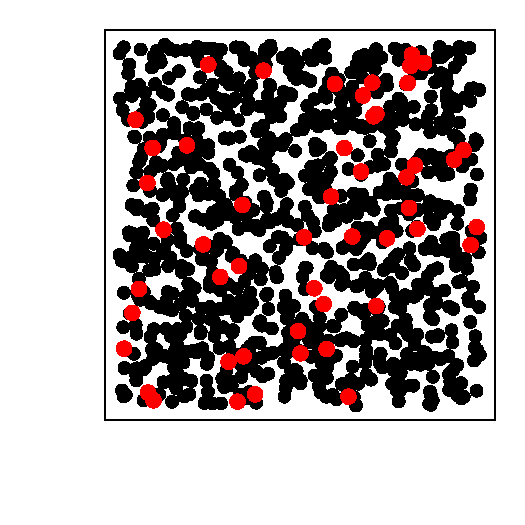
\includegraphics[width=.4\linewidth]{Figs/SquareLakeSample1-1} 
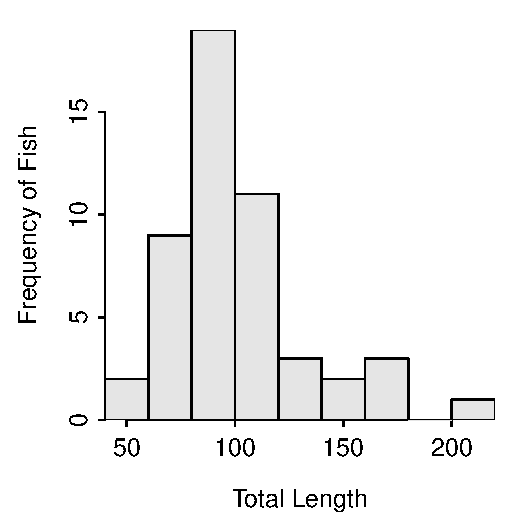
\includegraphics[width=.4\linewidth]{Figs/SquareLakeSample1-2} 

}

\caption{Schematic representation (\textbf{Left}) of a sample of 50 fish (i.e., red dots) from Square Lake and histogram (\textbf{Right}) of the total length of the 50 fish in this sample.}\label{fig:SquareLakeSample1}
\end{figure}


\end{knitrout}

Summaries computed from individuals in a sample are called \textbf{statistics}.\index{Statistic!Definition}  Specific names of statistics are preceded by ``sample.''  The statistic of interest is always the same as the parameter of interest; i.e., the statistic describes the sample in the same way that the parameter describes the population. For example, if interest is in the population mean, then the sample mean would be computed.

Some statistics computed from the sample from Square Lake are shown in \tabref{tab:SquareLakeSample1} and \figref{fig:SquareLakeSample1}. The sample mean of 100.04 mm is the best ``guess'' at the population mean. Not surprisingly from the discussion in \modref{chap:WhyStatsImportant}, the sample mean does not perfectly equal the population mean.

% latex table generated in R 3.4.0 by xtable 1.8-2 package
% Sun May 21 17:06:39 2017
\begin{table}[ht]
\centering
\caption{Summary statistics for the total length of a sample of 50 fish from the Square Lake population.} 
\label{tab:SquareLakeSample1}
\begin{tabular}{cccccccc}
 n & mean & sd & min & Q1 & median & Q3 & max \\ 
  \hline
50 & 100.04 & 31.94 & 49 & 81 & 91 & 118 & 203 \\ 
   \hline
\end{tabular}
\end{table}


\warn{An individual is not necessarily a person.}

\vspace{-12pt}
\warn{Populations and parameters can generally not be ``seen.''}


\section{Performing an IVPPSS}
In each statistical analysis it is important that you determine the Individual, Variable, Population, Parameter, Sample, and Statistic (\textbf{IVPPSS}). First, determine what items you are actually going to look at; those are the individuals. Second, determine what is recorded about each individual; that is the variable. Third, ALL individuals is the population. Fourth, the summary (e.g., mean or proportion) of the variable recorded from ALL individuals in the population is the parameter.\footnote{Again, parameters generally cannot be computed because all of the individuals in the population can not be seen. Thus, the parameter is largely conceptual.} Fifth, the population usually cannot be seen, so only a few individuals are examined; those few individuals are the sample. Finally, the summary of the individuals in the sample is the statistic.

When performing an IVPPSS, keep in mind that parameters describe populations (note that they both start with ``p'') and statistics describe samples (note that they both start with ``s''). This can also be looked at from another perspective. A sample is an estimate of the population and a statistic is an estimate of a parameter. Thus, the statistic has to be the same summary (mean or proportion) of the sample as the parameter is of the population.

The IVPPSS process is illustrated for the following situation:
\vspace{-6pt}
\begin{quote}
\textit{A University of New Hampshire graduate student (and Northland College alum) investigated habitat utilization by New England (Sylvilagus transitionalis) and Eastern (Sylvilagus floridanus) cottontail rabbits in eastern Maine in 2007. In a preliminary portion of his research he determined the proportion of ``rabbit patches'' that were inhabited by New England cottontails. He examined 70 ``patches'' and found that 53 showed evidence of inhabitance by New England cottontails.}
\end{quote}
\vspace{-6pt}

\begin{Itemize}
  \item An individual is a rabbit patch in eastern Maine in 2007 (i.e., a rabbit patch is the ``item'' being sampled and examined).
  \item The variable is ``evidence for New England cottontails or not (yes or no)'' (i.e., the characteristic of each rabbit patch that was recorded).
  \item The population is ALL rabbit patches in eastern Maine in 2007.
  \item The parameter is the proportion of ALL rabbit patches in eastern Maine in 2007 that showed evidence for New England cottontails.\footnote{Note that this population and parameter cannot actually be calculated but it is what the researcher wants to know.}
  \item The sample is the 70 rabbit patches from eastern Maine in 2007 that were actually examined by the researcher.
  \item The statistic is the proportion of the 70 rabbit patches from eastern Maine in 2007 actually examined that showed evidence for New England cottontails. [In this case, the statistic would be 53/70 or 0.757.]
\end{Itemize}

In the descriptions above, take note that the individual is very carefully defined (including stating a specific time (2007) and place (eastern Maine)), the population and parameter both use the word ``ALL'', the sample and statistic both use the specific sample size (70 rabbits), and that the parameter and statistics both use the same summary (i.e., proportion of patches that showed evidence of New England cottontails).

In some situations it may be easier to identify the sample first. From this, and realizing that a sample is always ``of the individuals,'' it may be easier to identify the individual. This process is illustrated in the following example, with the items listed in the order identified rather than in the traditional IVPPSS order.

\vspace{-6pt}
\begin{quote}
\textit{The Duluth, MN Touristry Board is interested in the average number of raptors seen per year at Hawk Ridge.\footnote{Information about Hawk Ridge is found \href{http://www.hawkridge.org/}{here}.}  To determine this value, they collected the total number of raptors seen in a sample of years from 1971-2003.}
\end{quote}
\vspace{-6pt}

\begin{Itemize}
  \item The sample is the 32 years between 1971 and 2003 at Hawk Ridge.
  \item An individual is a year (because a ``sample of \emph{years}'' was taken) at Hawk Ridge.
  \item The variable recorded was the number of raptors seen in one year at Hawk Ridge.
  \item The population is ALL years at Hawk Ridge (this is a bit ambiguous but may be thought of as all years that Hawk Ridge has existed).
  \item The parameter is the average number of raptors seen per year in ALL years at Hawk Ridge.
  \item The statistic is the average number of raptors seen in the 1971-2003 sample of years at Hawk Ridge.
\end{Itemize}

Again, note that the individual is very carefully defined (including stating a specific time and place), the population and parameter both use the word ``ALL'', the sample and statistic both use the specific sample size (32 years), and that the parameter and statistics both use the same summary (i.e., average number of raptors).

\warn{An individual is usually defined by a specific time and place.}

\vspace{-12pt}
\warn{Descriptions for population and parameter will always include the word ``All.''}

\vspace{-12pt}
\warn{Descriptions for sample and statistic will contain the specific sample size.}

\vspace{-12pt}
\warn{Descriptions for parameter and statistic will contain the same summary (usually average/mean or proportion/percentage). Howeve the summary is for a different set of individuals -- the population for the parameter and the sample for the statistic.}


\subsection{Sampling Variability (Revisited)}
It is instructive to once again (see \modref{chap:WhyStatsImportant}) consider how statistics differ among samples. \tabref{tab:SquareLakeSample234} and \figref{fig:SquareLakeSample234} show results from three more samples of n=50 fish from the Square Lake population. The means from all four samples (including the sample in \tabref{tab:SquareLakeSample1} and \figref{fig:SquareLakeSample1}) were quite different from the known population mean of 98.06 mm. Similarly, all four histograms were similar in appearance but slightly different in actual values. These results illustrate that a statistic (or sample) will only approximate the parameter (or population) and that statistics vary among samples. This \textbf{sampling variability} is one of the most important concepts in statistics and is discussed in great detail beginning in \modref{chap:SamplingDist}.\index{Sampling Variability!Definition}

\begin{knitrout}
\definecolor{shadecolor}{rgb}{0.922, 0.922, 0.922}\color{fgcolor}\begin{figure}[hbtp]

{\centering 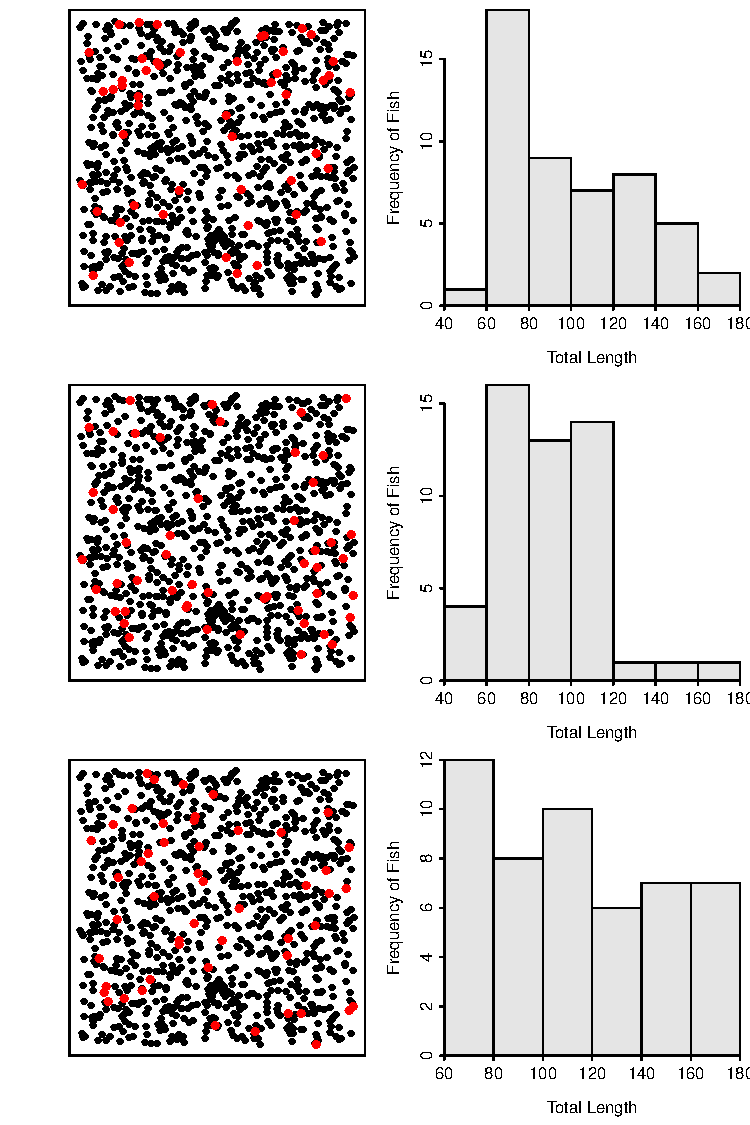
\includegraphics[width=.7\linewidth]{Figs/SquareLakeSample234-1} 

}

\caption{Schematic representation (\textbf{Left}) of three samples of 50 fish (i.e., red dots) from Square Lake and histograms (\textbf{Right}) of the total length of the 50 fish in each sample.}\label{fig:SquareLakeSample234}
\end{figure}


\end{knitrout}

% latex table generated in R 3.4.0 by xtable 1.8-2 package
% Sun May 21 17:06:40 2017
\begin{table}[htbp]
\centering
\caption{Summary statistics for the total length in three samples of 50 fish from the Square Lake population.} 
\label{tab:SquareLakeSample234}
\begin{tabular}{cccccccc}
 n & mean & sd & min & Q1 & median & Q3 & max \\ 
  \hline
50 & 99.56 & 32.47 & 57 & 69 & 91 & 123 & 167 \\ 
  50 & 88.64 & 24.52 & 53 & 68 & 86 & 106 & 166 \\ 
  50 & 112.74 & 35.86 & 61 & 84 & 108 & 147 & 174 \\ 
   \hline
\end{tabular}
\end{table}


%\defn{Sampling Variability}{The realization that no two samples are exactly alike. Thus, statistics computed from different samples will likely vary.}

This example also illustrates that parameters are fixed values because populations don't change. If a population does change, then it is considered a different population. In the Square Lake example, if a fish is removed from the lake, then the fish in the lake would be considered a different population. Statistics, on the other hand, vary depending on the sample because each sample consists of different individuals that vary (i.e., sampling variability exists because natural variability exists).

\warn{Parameters are fixed in value, while statistics vary in value.}


\section{Variable Types}\label{sect:VarTypes}
The type of statistic that can be calculated is dictated by the type of variable recorded. For example, an average can only be calculated for quantitative variables (defined below). Thus, the type of variable should be identified immediately after performing an IVPPSS.

\subsection{Variable Definitions}
There are two main groups of variable types -- quantitative and categorical \figrefp{fig:VarTypes}. \textbf{Quantitative} variables are variables with numerical values for which it makes sense to do arithmetic operations (like adding or averaging).\index{Quantitative Variable}  Synonyms for quantitative are measurement or numerical. \textbf{Categorical} variables are variables that record which group or category an individual belongs.\index{Categorical Variable}  Synonyms for categorical are qualitative or attribute. Within each main type of variable are two subgroups \figrefp{fig:VarTypes}.

\begin{knitrout}
\definecolor{shadecolor}{rgb}{0.922, 0.922, 0.922}\color{fgcolor}\begin{figure}[hbtp]

{\centering 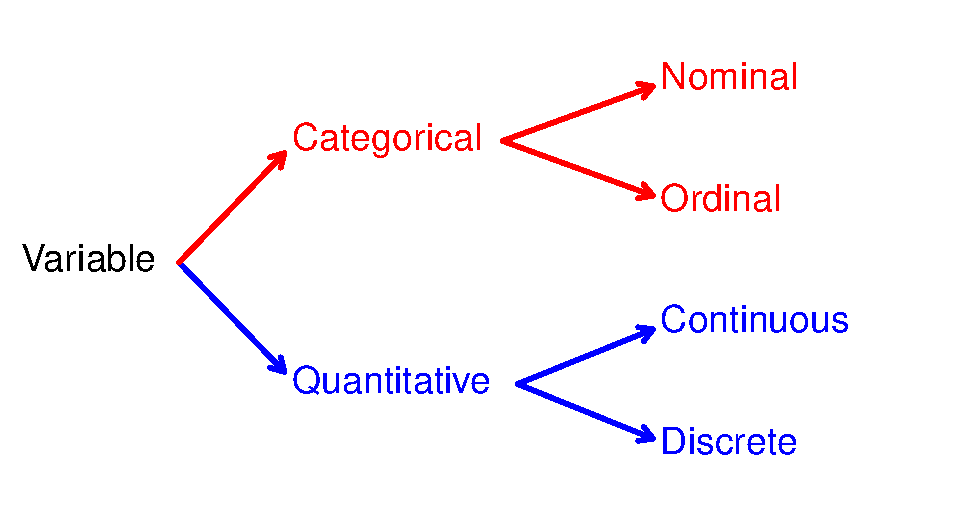
\includegraphics[width=.5\linewidth]{Figs/VarTypes-1} 

}

\caption[Schematic representation of the four types of variables]{Schematic representation of the four types of variables.}\label{fig:VarTypes}
\end{figure}


\end{knitrout}
\vspace{9pt} % added because of paragraph compressions following R code

The two types of quantitative variables are continuous and discrete variables. \textbf{Continuous} variables are quantitative variables that have an uncountable number of values.\index{Continuous Variable}  In other words, a potential value \textsc{does} exist between every pair of values of a continuous variable. \textbf{Discrete} variables are quantitative variables that have a countable number of values.\index{Discrete Variable}  Stated differently, a potential value \textsc{does not} exist between every pair of values for a discrete variable. Typically, but not always, discrete variables are counts of items.

Continuous and discrete variables are easily distinguished by determining if it is possible for a value to exist between every two values of the variable. For example, can there be between 2 and 3 ducks on a pond?  No!  Thus, the number of ducks is a discrete variable. Alternatively, can a duck weigh between 2 and 3 kg?  Yes!  Can it weigh between 2 and 2.1 kg?  Yes!  Can it weigh between 2 and 2.01 kg?  Yes!  You can see that this line of questions could continue forever; thus, duck weight is a continuous variable.

\warn{A quantitative variable is continuous if a possible value exists between every two values of the variable; otherwise, it is discrete.}

The two types of categorical variables are ordinal and nominal. \textbf{Ordinal} variables are categorical variables where a natural order or ranking exists among the categories.\index{Ordinal Variable}  \textbf{Nominal} variables are categorical variables where no order or ranking exists among the categories.\index{Nominal Variable}

Ordinal and nominal variables are easily distinguished by determining if the order of the categories matters. For example, suppose that a researcher recorded a subjective measure of condition (i.e., poor, average, excellent) and the species of each duck. Order matters with the condition variable -- i.e., condition improves from the first (poor) to the last category (excellent) -- and some reorderings of the categories would not make sense -- i.e., average, poor, excellent does not make sense. Thus, condition is an ordinal variable. In contrast, species (e.g., mallard, redhead, canvasback, and wood duck) is a nominal variable because there is no inherent order among the categories (i.e., any reordering of the categories also ``makes sense'').

\warn{\textbf{Ord}inal means that an \textbf{ord}er among the categories exists (note ``ord'' in both ordinal and order).}

The following are some issues to consider when identifying the type of a variable:
\begin{Enumerate}
  \item The categories of a categorical variable are sometimes labeled with numbers. For example, 1=``Poor'', 3=``Fair'', and 5=``Good''. Don't let this fool you into calling the variable quantitative.
  \item Rankings, ratings, and preferences are ordinal (categorical) variables.
  \item Counts of numbers are discrete (quantitative) variables.
  \item Measurements are typically continuous (quantitative) variables.
  \item It does not matter how precisely quantiative variables are recorded when deciding if the variable is continuous or discrete. For example, the weight of the duck might have been recorded to the nearest kg. However, this was just a choice that was made, the actual values can be continuously finer than kg and, thus, weight is a continuous variable.
  \item Categorical variables that consist of only two levels or categories will be labeled as a nominal variable (because any order of the groups makes sense). This type of variable is also often called ``binomial.''
  \item Do not confuse ``what type of variable'' (answer is one of ``continuous'', ``discrete'', ``nominal'', or ``ordinal'')  with ``what type of variability'' (answer is ``natural'' or ``sampling'') questions.
\end{Enumerate}

\warn{``What type of variable is ...?'' is a different question than ``what type of variability is ...?''  Be careful to note the word difference (i.e., ``variable'' versus ``variability'') when answering these questions.}

\vspace{-12pt}
\warn{The precision to which a quantitative variable was recorded does not determine whether it is continuous or discrete. How precisely the variable COULD have been recorded is the important consideration.}



\chapter{Data Production} \label{chap:DataProd}
\begin{ChapObj}{\boxwidth}
  \textbf{Objectives:}
  \begin{Enumerate}
    \item Identify major differences between data produced from experiments and observational studies.
    \item Understand basic ideas of simple random experiments with one and two factors.
    \item Describe the principles of experimental design.
    \item Describe the principles of observational studies.
    \item Understand basic ideas of designing simple observational studies, and
    \item Explain the importance of randomization in both experiments and observational studies.
  \end{Enumerate}
\end{ChapObj}

\minitoc
\newpage

\lettrine{S}{tatistical inference is the process} of making conclusions about a population from the results of a single sample.\index{Inference!Definition} To make conclusions about the larger population, the sample must fairly represent the larger population. Thus, the proper collection (or production) of data is critical to statistics (and science in general). In this module, two ways of producing data -- (1) Experiments and (2) Observational Studies -- are described.

\warn{Inferences cannot be made if data are not properly collected.}


\section{Experiments}
An experiment deliberately imposes a \textit{condition} on individuals to observe the effect on the \textbf{response variable}.\index{Experiment!Definition}\index{Response Variable!Experiment} In a properly designed experiment, all variables that are not of interest are held constant, whereas the variable(s) that is (are) of interest are changed among treatments. As long as the experiment is designed properly (see below), differences among treatments are either due to the variable(s) that were deliberately changed or randomness (chance). Methods to determine if differences were likely due to randomness are developed in later modules. Because we can determine if differences most likely occurred o randomness or changes in the variales, strong \textit{cause-and-effect conclusions} can be made from data collected from carefully designed experiments.

\subsection{Single-factor Experiments}\index{Experiment!Single-Factor}
A \textbf{factor} is a variable that is deliberately manipulated to determine its effect on the response variable.\index{Factor!Experiment} A factor is sometimes called an \textbf{explanatory variable} because we are attempting to determine how it affects (or ``explains'') the response variable. The simplest experiment is a single-factor experiment where the individuals are split into groups defined by the categories of a single factor.

For example, suppose that a researcher wants to examine the effect of temperature on the total number of bacterial cells after two weeks. They have inoculated 120 agars\footnote{An agar, in this case, is a petri dish with a growth medium for the bacteria.} with the bacteria and placed them in a chamber where all environmental conditions (e.g., temperature, humidity, light) are controlled exactly. The researchers will use only two temperatures in this simple experiment -- $10^{o}$C and $15^{o}$C. All other variables are maintained at constant levels. Thus, temperature is the only factor in this simple experiement because it is the only variable manipulated to different values to determine its impact on the number of bacterial cells.

\warn{In a single-factor experiment only one explanatory variable (i.e., factor) is allowed to vary; all other explanatory variables are held constant.}

\textbf{Levels} are the number of categories of the factor variable.\index{Level!Experimental} In this example, there are two levels -- $10^{o}$C and $15^{o}$C. \textbf{Treatments} are the number of unique conditions that individuals in the experiment are exposed to. In a single-factor experiment, the number of treatments is the same as the number of levels of the single factor.\index{Treatment, Experimental} Thus, in this simple experiment, there are two treatments -- $10^{o}$C and $15^{o}$C. Treatments are discussed more thoroughly in the next section.

The \textbf{number of replicates} in an experiment is the number of individuals that will receive each treatment.\index{Replicates} In this example, a replicate is an inoculated agar. The number of replicates is the number of inoculated agars that will receive each of the two temperature treatments. The number of replicates is determined by dividing the total number of available individuals (120) by the number of treatments (2). Thus, in this example, the number of replicates is 60 inoculated agars.

The agars used in this experiment will be randomly allocated to the two temperature treatments. All other variables -- humidity, light, etc. -- are kept the same for each treatment. At the end of two weeks, the total number of bacterial cells on each agar (i.e., the response variable) will be recorded and compared between the agars kept at both temperatures.\footnote{Methods for making this comparison are in \modref{chap:tTest2}.} Any difference in mean number of bacterial cells will be due to either different temperature treatments or randomness, because all other variables were the same between the two treatments.

\warn{Differences among treatments are either caused by randomness (chance) or the factor.}

The single factor is not restricted to just two levels. For example, more than two temperatures, say $10^{o}$C, $12.5^{o}$C, $15^{o}$C, and $17.5^{o}$C, could have been tested. With this modification, there is still only one factor -- temperature -- but there are now four levels (and only four treatments).

\subsection{Multi-factor Experiments -- Design and Definitions}
More than one factor can be tested in an experiment.\index{Experiment!Multi-Factor} In fact, it is more efficient to have a properly designed experiment where more than one factor is varied at a time than it is to use separate experiments in which only one factor is varied in each. However, before showing this benefit, let's examine the definitions from the previous section in a multi-factor experiment.

Suppose that the previous experiment was modified to also examine the effect of relative humidity on the number of bacteria cells. This modified experiment has two factors -- temperature (with two levels of $10^{o}$C or $15^{o}$C) and relative humidity (with four levels of 20\%, 40\%, 60\%, and 80\%). The number of treatments, or combinations of all factors, in this experiment is found by multiplying the levels of all factors (i.e., 2$\times$4=8 in this case).\index{Treatment, Experimental} The number of replicates in this experiment is now 15 (i.e., total number of available agars divided by the number of treatments; 120/8).

\warn{The number of treatments is determined for the overall experiment, whereas the number of levels is determined for each factor.}

A drawing of the experimental design can be instructive (below). The drawing is a grid where the levels of one factor are the rows and the levels of the other factor are the columns. The number of rows and columns correspond to the levels of the two factors, respectively, whereas the number of cells in the grid is the number of treatments (numbered in this table to show eight treatments).

\begin{center}
\begin{tabular}{cc|c|c|c}
 & \multicolumn{4}{c}{Relative Humidity} \\
\cline{2-5}
 & 20\% & 40\% & 60\% & 80\% \\
\cline{2-5}
\multicolumn{1}{c|}{$10^{o}$C} & 1 & 2 & 3 & \multicolumn{1}{c|}{4} \\
\hline
\multicolumn{1}{c|}{$15^{o}$C} & 5 & 6 & 7 & \multicolumn{1}{c|}{8} \\
\cline{2-5}
\end{tabular}
\end{center}


\subsection{Multi-factor Experiments -- Benefits}
The analysis of a multi-factor experimental design is more involved than what will be shown in this course. However, multi-factor experiments have many benefits, which can be illustrated by comparing a multi-factor experiment to separate single-factor experiments. For example, in addition to the two factor experiment in the previous section, consider separate single-factor experiments to determine the effect of each factor separately (further assume that individuals (i.e., agars) can be used in only one of these separate experiments).

To conduct the two separate experiments, randomly split the 120 available agars into two equally-sized groups of 60. The first 60 will be split into two groups of 30 for the first experiment with two temperatures. The second 60 will be split into four groups of 15 for the second experiment with four relative humidities. These separate single-factor experiments are summarized in the following tables (where the numbers in the cells represent the number of replicates in each treatment).

\begin{center}
\begin{tabular}{|c|c|c|c|c|c|c|}
\multicolumn{2}{c}{Temperature} & \multicolumn{1}{c}{} & \multicolumn{4}{c}{Relative Humidity} \\
\cline{1-2}\cline{4-7}
$10^{o}$C & $15^{o}$C & & 20\% & 40\% & 60\% & 80\% \\
\cline{1-2}\cline{4-7}
30 & 30 & & 15 & 15 & 15 & 15 \\
\cline{1-2}\cline{4-7}
\end{tabular}
\end{center}

The tabel below was modified from the previous section to show the number of replicates in each treatment of the experiment where both factors were simultaneously manipulated.

\begin{center}
\begin{tabular}{cc|c|c|c}
 & \multicolumn{4}{c}{Relative Humidity} \\
\cline{2-5}
 & 20\% & 40\% & 60\% & 80\% \\
\cline{2-5}
\multicolumn{1}{c|}{$10^{o}$C} & 15 & 15 & 15 & \multicolumn{1}{c|}{15} \\
\hline
\multicolumn{1}{c|}{$15^{o}$C} & 15 & 15 & 15 & \multicolumn{1}{c|}{15} \\
\cline{2-5}
\end{tabular}
\end{center}

The key to examining the benefits of the multi-factor experiment is to determine the number of individuals that give ``information'' about (i.e., are exposed to) each factor. From the last table it is seen that all 120 individuals were exposed to one of the temperature levels with 60 individuals exposed to each level. In contrast, only 30 individuals were exposed to these levels in the single-factor experiment. In addition, all 120 individuals were exposed to one of the relative humidity levels with 30 individuals exposed to each level. Again, this is in contrast to the single-factor experiment where only 15 individuals were exposed to these levels. Thus, the first advantage of multi-factor experiments is that the available individuals are used more efficiently. In other words, more ``information'' (i.e., the responses of more individuals) is obtained from a multi-factor experiment than from combinations of single-factor experiments.\footnote{The real importance of this advantage will become apparent when statistical power is introduced in \modref{chap:HypothesisTests}.}

A properly designed multi-factor experiment also allows researchers to determine if multiple factors interact to impact an individual's response.\index{Interaction effect} For example, consider the hypothetical results from this experiment in \figref{fig:ExpDInt}.\footnote{The means of each treatment are plotted and connected with lines in this plot.} The effect of relative humidity is to increase the growth rate for those individuals at $10^{o}$C (black line) but to decrease the growth rate for those individuals at $15^{o}$C (blue line). That is, the effect of relative humidity differs depending on the level of temperature. When the effect of one factor differs depending on the level of the other factor, then the two factors are said to \textit{interact}. Interactions cannot be determined from the two single-factor experiments because the same individuals are not exposed to levels of the two factors at the same time.

\begin{knitrout}
\definecolor{shadecolor}{rgb}{0.922, 0.922, 0.922}\color{fgcolor}\begin{figure}[hbtp]

{\centering 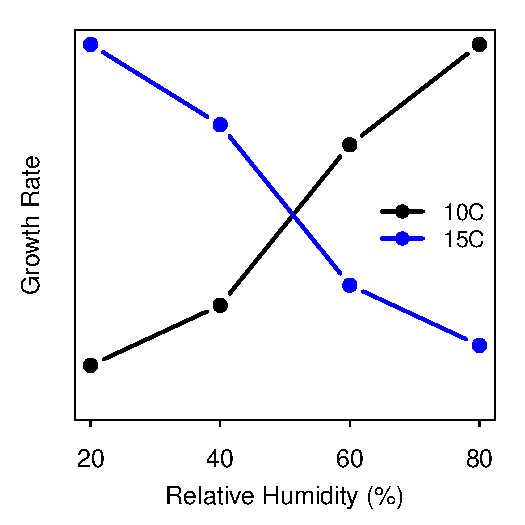
\includegraphics[width=.4\linewidth]{Figs/ExpDInt-1} 

}

\caption[Mean growth rates in a two-factor experiment that depict an interaction effect]{Mean growth rates in a two-factor experiment that depict an interaction effect.}\label{fig:ExpDInt}
\end{figure}


\end{knitrout}
\vspace{9pt} % added because of paragraph compressions following R code

Multi-factor experiments are used to detect the presence or absence of interaction, not just the presence of it. The hypothetical results in \figref{fig:ExpDNoInt} show that the growth rate increases with increasing relative humidity at about the same rate for both temperatures. Thus, because the effect of relative humidity is the same for each temperature (and vice versa), there does not appear to be an interaction between the two factors. Again, this could not be determined from the separate single-factor experiments.

\begin{knitrout}
\definecolor{shadecolor}{rgb}{0.922, 0.922, 0.922}\color{fgcolor}\begin{figure}[hbtp]

{\centering 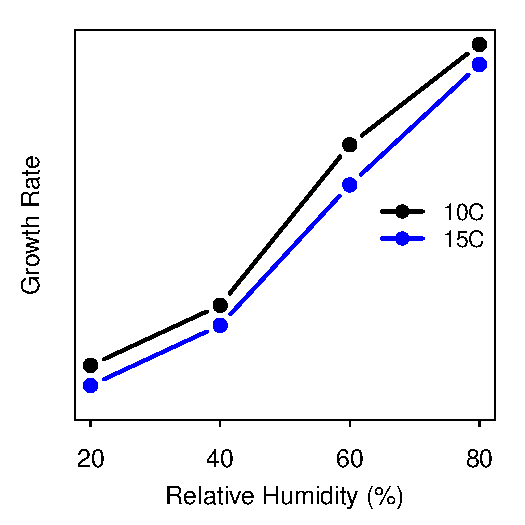
\includegraphics[width=.4\linewidth]{Figs/ExpDNoInt-1} 

}

\caption[Mean growth rates in a two-factor experiment that depict no interaction effect]{Mean growth rates in a two-factor experiment that depict no interaction effect.}\label{fig:ExpDNoInt}
\end{figure}


\end{knitrout}


\subsection{Allocating Individuals}
Individuals\footnote{When discussing experiments, an ``individual'' is often referred to as a ``replicate'' or an ``experimental unit.''} should be randomly allocated (i.e., placed into) to treatments.\index{Replicates} Randomization will tend to even out differences among groups for variables not considered in the experiment. In other words, randomization should help assure that all groups are similar before the treatments are imposed. Thus, randomly allocating individuals to treatments removes any bias (foreseen or unforeseen) from entering the experiment.

In the single-factor experiment above -- two treatments of temperature -- there were 120 agars. To randomly allocate these individuals to the treatments, 60 pieces of paper marked with ``10'' and 60 marked with ``15'' could be placed into a hat. One piece of paper would be drawn for each agar and the agar would receive the temperature found on the piece of paper. Alternatively, each agar could be assigned a unique number between 1 and 120 and pieces of paper with these numbers could be placed into the hat. Agars corresponding to the first 60 numbers drawn from the hat could then be placed into the first treatment. Agars for the next (or remaining) 60 numbers would be placed in the second treatment. This process is essentially the same as randomly ordering 120 numbers.

A random order of numbers is obtained with R by including the count of numbers as the only argument to \R{sample()}. For example, randomly ordering 1 through 120 is accomplished with

\begin{knitrout}
\definecolor{shadecolor}{rgb}{0.922, 0.922, 0.922}\color{fgcolor}\begin{kframe}
\begin{verbatim}
> sample(120)
\end{verbatim}
\end{kframe}
\end{knitrout}
\vspace{-12pt}
\begin{knitrout}
\definecolor{shadecolor}{rgb}{0.922, 0.922, 0.922}\color{fgcolor}\begin{kframe}
\begin{verbatim}
  [1]  80  30 100  90  21  68 104  79  64 106  98  16  73  91 107   1  60  54  26  99
 [21] 108 111  31  47  57  92   5  58  37  50  34  88  41  66  65  29 110 113   4  75
 [41]  93  23  49  97  35  84  74   7  15  39  70  94 114  14  71  20  33  67  86   8
 [61]   6  28  52  48  13  18  63  72  69 120  55  83  42   3  77  82  38  22  96  43
 [81]  56  89  78  17 112  44 103  46  59  85 109 115 118  87  32  62  51  95  24  40
[101] 119 102  19  27 116  36   2  12  45  53  11  76 117  61 105   9 101  25  81  10
\end{verbatim}
\end{kframe}
\end{knitrout}

Thus, the first five (of 60) agars in the 10$^{o}$C treatment are 80, 30, 100, 90, and 21. The first five (of 60) agars in the 15$^{o}$C treatment are 6, 28, 52, 48, and 13.

In the modified experiment with two factors -- temperature and relative humidity -- with eight treatments containing 15 agars each, it is more efficient to save the random numbers into an object and then select the numbers in the first 15 positions, then the second 15 positions, etc. Positions are selected from an object by putting the position numbers in square brackets following the object name. Additionally, a colon is used to make a sequence of integers from the number before to the number after the colon.\footnote{For example, \R{1:4} will make an object with the numbers 1, 2, 3, and 4 in it.}
\begin{knitrout}
\definecolor{shadecolor}{rgb}{0.922, 0.922, 0.922}\color{fgcolor}\begin{kframe}
\begin{verbatim}
> ragars2 <- sample(120)
> ragars2[1:15]     # "grab" the first 15 numbers
 [1]  61  82 103  31  66  81 105  40 104 106   5   9  71  36   8
> ragars2[16:30]    # "grab" the second 15 numbers, and so on
 [1] 120   6  26  41  62 111  83  20  57   1  63  86  70  85  73
\end{verbatim}
\end{kframe}
\end{knitrout}

This design might be shown with the following table, where the numbers in each cell represent the first two agars selected to receive that treatment.\footnote{Only the first two numbers are shown because of space constraints.}

\begin{center}
\begin{tabular}{cc|c|c|c}
 & \multicolumn{4}{c}{Relative Humidity} \\
\cline{2-5}
 & 20\% & 40\% & 60\% & 80\% \\
\cline{2-5}
\multicolumn{1}{c|}{$10^{o}$C} & 61,82,$\cdots$ & 120,6,$\cdots$ & 60,72,$\cdots$ & \multicolumn{1}{c|}{89,49,$\cdots$} \\
\hline
\multicolumn{1}{c|}{$15^{o}$C} & 78,10,$\cdots$ & 109,101,$\cdots$ & 22,2,$\cdots$ & \multicolumn{1}{c|}{114,77,$\cdots$} \\
\cline{2-5}
\end{tabular}
\end{center}

\warn{Individuals should be randomly allocated to treatments to remove bias.}


\subsection{Design Principles}
There are many other methods of designing experiments and allocating individuals that are beyond the scope of this book.\footnote{Other common designs include blocked, Latin square, and nested designs.} However, all experimental designs contain the following three basic principles.\index{Experiment!Principles}
\begin{Enumerate}
  \item \textbf{Control} the effect of variables on the response variable by deliberately manipulating factors to certain levels and maintaining constancy among other variables.
  \item \textbf{Randomize} the allocation of individuals to treatments to eliminate bias.
  \item \textbf{Replicate individuals} (use many individuals) in the experiment to reduce chance variation in the results.
\end{Enumerate}

Proper control in an experiment allows for strong cause-and-effect conclusions to be made (i.e., to state that an observed difference in the response variable was due to the levels of the factor or chance variation rather than some other foreseen or unforeseen variable). Randomly allocating individuals to treatments removes any bias that may be included in the experiment. For example, if we do not randomly allocate the agars to the treatments, then it is possible that a set of all ``poor'' agars may end up in one treatment. In this case, any observed differences in the response may not be due to the levels of the factor but to the prior quality of the agars. Replication means that there should be more than one or a few individuals in each treatment. This reduces the effect of each individual on the overall results. For example, if there was one agar in each treatment, then, even with random allocation, the effect of that treatment may be due to some inherent properties of that agar rather than the levels of the factors. Replication, along with randomization, helps assure that the groups of individuals in each treatment are as alike as possible at the start of the experiment.


\section{Observational Studies -- Sampling}
In observational studies the researcher has no control over any of the variables observed for an individual.\index{Observational Study} The researcher simply observes individuals, disturbing them as little as possible, trying to get a ``picture'' of the population. Observational studies cannot be used to make cause-and-effect statements because all variables that may impact the outcome may not have been measured or specifically controlled. Thus, any observed difference among groups may be caused by the variables measured, some other unmeasured variables, or chance (randomness).

Consider the following as an example of the problems that can occur when all variables are not measured. For many years scientists thought that the brains of females weighed less than the brains of males. They used this finding to support all kinds of ideas about sex-based differences in learning ability. However, these earlier researchers failed to measure body weight, which is strongly related to brain weight in both males and females. After controlling for the effect of differences in body weights, there was no difference in brain weights between the sexes. Thus, many sexist ideas persisted for years because cause-and-effect statements were inferred from data where all variables were not considered.

\warn{Strong cause-and-effect statements CANNOT be made from observational studies.}

In observational studies, it is important to understand to which population inferences will refer.\footnote{Thus, it is very important to first perform an IVPPS as discussed in \modref{chap:FoundationalDefinitions}.} To make useful inferences from a sample, the sample must be an unbiased representation of the population. In other words, it must not systematically favor certain individuals or outcomes.

For example, consider that you want to determine the mean length of all fish in a particular lake (e.g., Square Lake from \modref{chap:FoundationalDefinitions}). Using a net with large mesh, such that only large fish are caught, would produce a biased sample because interest is in all fish not just the large fish. Setting the nets near spawning beds (i.e., only adult fish) would also produce a biased sample. In both instances, a sample would be collected from a population other than the population of interest. Thus it is important to select a sample from the specified population.

\warn{It is important to understand the population before considering how to take a sample.}

\subsection{Types of Sampling Designs}
Three common types of sampling designs -- voluntary response, convenience, and probability-based samples -- are considered in this section. Voluntary response and convenience samples tend to produce biased samples, whereas proper probability-based samples will produce an unbiased sample.

A \textbf{voluntary response} sample consists of individuals that have chosen themselves for the sample by responding to a general appeal.\index{Voluntary Response Sample} An example of a voluntary response sample would be the group of people that respond to a general appeal placed in the school newspaper. If the population of interest in this sample was all students at the school, then this type of general appeal would likely produce a biased sample of students that (i) read the school newspaper, (ii) feel strongly about the topic, or (iii) both.

A \textbf{convenience} sample consists of individuals who are easiest to reach for the researcher.\index{Convenience Sample} An example of a convenience sample is when a researcher queries only those students in a particular class. This sample is ``convenient'' because the individuals are easy to gather. However, if the population of interest was all students at the school, then this type of sample would likely produce a biased sample of students that is likely of (i) one major or another, (ii) one or a few ``years-in-school'' (e.g., Freshman or Sophomores), or (iii) both.

In probability-based sampling, each individual of the population has a known chance of being selected for the sample. The simplest probability-based sample is the \textbf{Simple Random Sample} (SRS) where each individual has the same chance of being selected.\index{Simple Random Sample} Proper selection of an SRS requires each individual to be assigned a unique number. The SRS is then formed by choosing random numbers and collecting the individuals that correspond to those numbers.

For example, an auditor may need to select a sample of 30 financial transactions from all transactions of a particular bank during the previous month. Because each transaction is numbered, the auditor may know that there were 1112 transactions during the previous month (i.e., the population). The auditor would then number each transaction from 1 to 1112, randomly select 30 numbers (with no repeats) from between 1 and 1112, and then physically locate the 30 transactions that correspond to the 30 selected numbers. Those 30 transactions are the SRS.

Random numbers are selected in R by including the population size as the first and sample size as the second argument to \R{sample()}. For example, 30 numbers from between 1 and 1112 is selected with

\begin{knitrout}
\definecolor{shadecolor}{rgb}{0.922, 0.922, 0.922}\color{fgcolor}\begin{kframe}
\begin{verbatim}
> sample(1112,30)
\end{verbatim}
\end{kframe}
\end{knitrout}
\vspace{-12pt}
\begin{knitrout}
\definecolor{shadecolor}{rgb}{0.922, 0.922, 0.922}\color{fgcolor}\begin{kframe}
\begin{verbatim}
 [1]   75  320  874  104  128  870  607 1091 1030 1053 1031  518  433  893  816  903
[17]  342 1016  136  580  670  376  576 1076 1034  365  492  189  409   66
\end{verbatim}
\end{kframe}
\end{knitrout}

Thus, accounts 75, 320, 874, 104, and 128 would be the first five (of 30) selected.

There are other more complex types of probability-based samples that are beyond the scope of this course.\footnote{For example, stratified samples, nested, and multistage samples.} However, the goal of these more complex types of samples is generally to impart more control into the sampling design.

\warn{A proper SRS requires each individual i the population to be assigned a unique number.}

If the population is such that a number cannot be assigned to each individual, then the researcher must try to use a method for which they feel each individual has an equal chance of being selected. Usually this means randomizing the technique rather than the individuals. In the fish example discussed on the previous page, the researcher may consider choosing random mesh sizes, random locations for placing the net, or random times for placing the net. Thus, in many real-life instances, the researcher simply tries to use a method that is likely to produce an SRS or something very close to it.

\warn{If a number cannot be assigned to each individual in the population, then the researcher should randomize the ``technique'' to assure as close to a random sample as possible.}

Polls, campaign or otherwise, are examples of observational studies that you are probably familiar with. The following are links where various aspects of polling are discussed.
\begin{Itemize}
  \item \href{http://media.gallup.com/PDF/FAQ/HowArePolls.pdf}{How Polls are Conducted by Frank Newport, Lydia Saad, and David Moore, The Gallup Organization}.
  \item \href{http://www2.psych.purdue.edu/~codelab/Invalid.Polls.html}{Why Do Campaign Polls Zigzag So Much? by G.S. Wasserman, Purdue U}.
\end{Itemize}


\subsection{Of What Value are Observational Studies?}
Properly designed experiments can lead to ``cause-and-effect'' statements, whereas observational studies (even properly designed) are unlikely to lead to such statements. Furthermore, in the last section, it was suggested that it is very difficult to take a proper probability-based sample because it is hard to assign a number to each individual in the population (precisely because entire populations are very difficult to ``see''). So, do observational studies have any value?  There are at least three reasons why observational studies are useful.

The scientific method begins with making an observation about a natural phenomenon. Observational studies may serve to provide such an observation. Alternatively, observational studies may be deployed after an observation has been made to see if that observation is ``prevalent'' and worthy of further investigation. Thus, observational studies may lead directly to hypotheses that form the basis of experiments.

Experiments are often conducted under very confined and controlled conditions so that the effect of one or more factors on the response variable can be identified. However, at the conclusion of an experiment it is often questioned whether a similar response would be observed ``in nature'' under much less controlled conditions. For example, one might determine that a certain fertilizer increases growth of a certain plant in the greenhouse, with consistent soil characteristics, temperatures, lighting, etc. However, it is a much different, and, perhaps, more interesting, question to determine if that fertilizer elicits the same response when applied to an actual field.

Finally, there are situations where conducting an experiment simply cannot be done, either for ethical, financial, size, or other constraints. For example, it is generally accepted that smoking causes cancer in humans even though an experiment where one group of people was forced to smoke while another was not allowed to smoke has not been conducted. Similarly, it is also very difficult to perform valid experiments on ``ecosystems.''  In these situations, an observational study is simply the best study allowable. Cause-and-effect statements are arrived at in these situations because observational studies can be conducted with some, though not absolute, control and control can be imparted mathematically into some analyses.\footnote{These analyses are beyond the scope of this book, though.} In addition, a ``preponderance of evidence'' may be arrived at if enough observational studies point to the same conclusion.



\chapter{Getting Started with R} \label{chap:FoundationsR}
\begin{ChapObj}{\boxwidth}
  \textbf{Objectives:}
  \begin{Enumerate}
    \item Understand the difference between R expressions and assignments.
    \item Understand the different types of data that can be stored in R.
    \item Understand the different types of data structures used in R.
    \item Be able to enter data into R data.frames.
    \item Be able to isolate individual variables and individuals in R.
    \item Be able to create data.frames that are subsets of larger data.frames.
    \item Understand how homework assignments should be formatted.
  \end{Enumerate}
\end{ChapObj}

\minitoc
\newpage

\section{Setting Up R and Helpers} \label{sect:RSetup}
\vspace{-8pt}
Detailed methods for downloading, installing, and configuring R, RStudio, and \R{NCStats} on your personal computer are given on the \href{http://derekogle.com/NCMTH107/resources/}{Resources page of the course website}.

\vspace{-8pt}
\section{Working With R Basics} \label{sect:RBasics}
\vspace{-12pt}
\subsection{Saving Results} \label{sect:RSaving}
Results are not saved in R or RStudio.  Rather, ``scripts'' of successful R commands are saved and, then, if the analysis needs to be re-done, the entire set of commands is opened in RStudio and run again.  When writing a report, all tabular and graphical output should be copied from RStudio and pasted into your report document.  This document will serve as your analysis report and can be modified to include answers to questions, references to the tables and graphs, etc.\footnote{Specifics for how to format homework assignments is on the course syllabus}  All data that is not a simple vector (see \sectref{sect:RVectors}) should be entered into R through text files (see \sectref{sect:REnterData}).

R does allow one to save a ``workspace'', though I urge you not to do that.  Rather, save your ``good'' commands in a script and save your ``good'' results in a report document; do not save the workspace.

\warn{Do NOT save the workspace in R.}

\vspace{-8pt}
\subsection{Expressions and Assignments} \label{sect:RExprAssn}
\vspace{-8pt}
Expressions in R are mathematical ``equations'' that are evaluated by R with a result seen immediately.  An example of an expression in R is
\begin{knitrout}
\definecolor{shadecolor}{rgb}{0.922, 0.922, 0.922}\color{fgcolor}\begin{kframe}
\begin{verbatim}
> 5+log(7)-pi
[1] 3.804317
\end{verbatim}
\end{kframe}
\end{knitrout}

where \R{log()} and \R{pi} are built-in functions used to compute the natural log and find the value of $\pi$, respectively.  Expressions in R are like using a calculator where the result is shown, but not saved for subsequent analyses.  In addition, expressions in R follow the same order of operations and use of parentheses as expressions entered into your calculator.

\warn{The results of expressions in R are temporary unless the result is assigned to an object.}

Results from an expression are typically saved for further computations by assigning the results of the expression to an object with the assignment operator (i.e., \R{<-}).  The general form for saving the result of an expression into an object is \R{object <- expression}.  The result of the expression will not be seen unless the object name is subsequently typed into R (but see below).  For example, the result of the previous expression is saved into an object called \R{x} and then viewed with
\begin{knitrout}
\definecolor{shadecolor}{rgb}{0.922, 0.922, 0.922}\color{fgcolor}\begin{kframe}
\begin{verbatim}
> x <- 5+log(7)-pi
> x
[1] 3.804317
\end{verbatim}
\end{kframe}
\end{knitrout}
The result of an expression can be both assigned and printed by surrounding the command in parentheses.  For example, the following assigns the result of the expression to \R{y} and prints the result.\footnote{The spaces between the expression and the parentheses are only needed to increase legibility.}
\begin{knitrout}
\definecolor{shadecolor}{rgb}{0.922, 0.922, 0.922}\color{fgcolor}\begin{kframe}
\begin{verbatim}
> ( y <- 15*exp(2) )
[1] 110.8358
\end{verbatim}
\end{kframe}
\end{knitrout}

\warn{The convention of surrounding commands in parentheses to both assign and print the results will be used extensively in this book to save space.}

An object can be named whatever you want, with the exception that it cannot start with a number, contain a space, or be the name of a reserved word or function in R (e.g., \R{pi} or \R{log}).  Furthermore, object names should be short and simple enough that you can remember what is contained in the object.  It is also good practice to view the object immediately after making the assignment to make sure that it contains results that seem appropriate.

\warn{In general, computational results should be assigned to an object.}

\vspace{-12pt}
\warn{Type the name of the object after making the assignment to confirm the results.}

\vspace{-8pt}
\begin{exsection}
  \item \label{revex:BasicsExpr1} \rhw{} Compute the value of $\frac{3}{7}+\frac{1}{2}$. \ansref{ans:BasicsExpr1}
  \item \label{revex:BasicsExpr2} \rhw{} Compute the value of $\pi*3.7^{2}$. \ansref{ans:BasicsExpr2}
  \item \label{revex:BasicsExpr3} \rhw{} Assign the value of 3.7 to \var{r}. \ansref{ans:BasicsExpr3}
  \item \label{revex:BasicsExpr4} \rhw{} Compute the value of $\pi r^{2}$ using the value of \var{r} assigned in the previous problem. \ansref{ans:BasicsExpr4}
  \item \label{revex:BasicsExpr5} \rhw{} \hspace{18pt} Assign the value 1.2 to \var{r} and then re-evaluate $\pi r^{2}$. \ansref{ans:BasicsExpr5}
\end{exsection}

\vspace{-18pt}
\subsection{Functions and Arguments}  \label{sect:RFunctions}
\vspace{-12pt}
R contains many ``programs,'' or functions, to perform particular tasks.  A function is ``called'' by typing the function name followed by open and closed parentheses.  Arguments, which the function will use to perform its task, are contained within the parentheses.  The \R{log()} function, used in the previous section, is an example of a function.  The name of the function is \R{log} and the argument, the number for which to compute the natural log, is contained within the parentheses following the function name.  Many other functions will be described below and in subsequent modules.

\defn{Function}{An R program that performs a particular task.}

\vspace{-12pt}
\defn{Argument}{A ``directive'' that is provided to a function.  Arguments are contained within parentheses that follow the function name.}

\vspace{-12pt}
\warn{Regular curved parentheses have two primary uses in R: (1) to control order of operations in expressions (as with a calculator) and (2) to contain the arguments sent to a function.}


\section{Working With Data}
\vspace{-12pt}
\subsection{Data Types}  \label{sect:RDataTypes}
\vspace{-12pt}
Data in R will be designated as an integer (whole numbers), numeric (non-integer numerica values), character (strings), factor (group membershop), or logical (TRUE/FALSE).  The type of data largely dictates the type of analysis that can be performed.  Data types will be discussed in more detail as needed.  Note, however, that the \textbf{factor} data type is a special case of the character data type, where the specific items describe the group to which an individual belongs.  This description allows for certain analyses in later modules.

\defn{Factor}{A special type of variable that identifies the group to which an individual belongs.}

\vspace{-12pt}
\subsection{Entering Data}  \label{sect:REnterData}
\vspace{-12pt}
For real data (i.e., several variables from many individuals) it is most efficient to enter data into a comma-separated values (CSV) file and then import that file into R.  Creating a CSV file with Microsoft Excel is described below, though there are other ways to create CSV files (see \href{http://derekogle.com/NCMTH107/resources/FAQ/}{FAQs on class webpage}).  This explanation assumes that you have a basic understanding of Excel (or other spreadsheet softwares).

\warn{Realistic datasets are most efficiently entered into a comma-separated values (CSV) file in preparation for importing into R.}

The spreadsheet should be organized with variables in columns and individuals in rows, with the exception that the first row should contain variable names.  The example spreadsheet below shows the length (cm), weight (kg), and capture location data for a small sample of Black Bears.

\begin{center}
  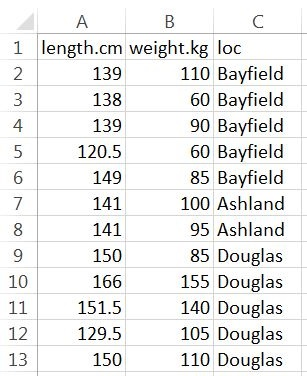
\includegraphics[width=1.5in]{Figs/Data_File_1.jpg}
\end{center}


\defn{data.frame}{A two-dimensional organization of variables (as columns, possibly of different data types) recorded on multiple individuals (as rows).}

\vspace{-12pt}
\warn{The columns of a data.frame correspond to variables and the rows of a data.frame correspond to individuals.}

Variable names must NOT contain spaces.  For example, don't use \var{total length} or \var{length (cm)}.  If you feel the need to have longer variable names, then separate the parts with a period (e.g., \var{length.cm}) or an underscore (e.g., \var{length\_cm}).  Furthermore, numerical measurements should NOT include units (e.g., don't use \verb"7 cm").  Finally, for categorical data, make sure that all categories are consistent (e.g., do not have a column that contains both \verb"bayfield" and \verb"Bayfield").

\warn{Variable names and data should not contain spaces.  An "\R{Error in scan}" message usually indicates spaces in the variable names or data.}

The spreadsheet is saved as a CSV file by selecting the \verb"File..Save As" menu item, which will produce the dialog box below. In this dialog box, change \verb"Save as type" to \verb"CSV (Comma delimited) (*.csv)" (you may have to scroll down), provide a file name (don't have any periods in the name besides for ``.csv'', which you should not have to type), select a location to save the file (don't forget this location!!), and press \verb"Save".  Two ``warning'' dialog boxes may then appear -- select \verb"OK" for the first and \verb"YES" for the second.  You can now close the spreadsheet file (you may be asked to save changes -- you should say \verb"No").
\begin{center}
  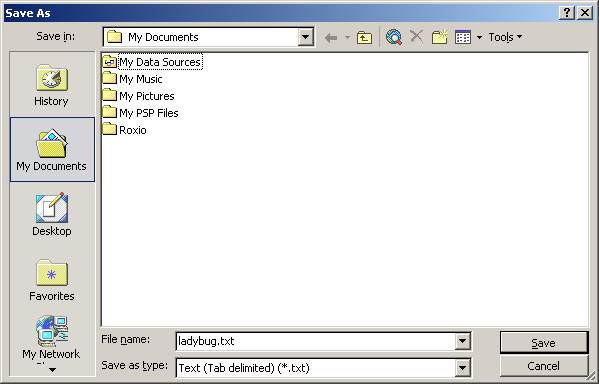
\includegraphics[width=3.5in]{Figs/Data_File_2.jpg}
\end{center}

The following steps are used to load the data in the CSV file into RStudio.

\begin{Itemize}
  \item Open RStudio.
  \item Open a new script by selecting the \verb"File", \verb"New File", \verb"R Script" menu items.
  \item Type \R{library(NCStats)} in the new script.
  \item Save this script by selecting the \verb"File", \verb"Save" menu items.  In the ensuing dialog box, navigate to the \textbf{exact same directory} where you saved the data, type a name for the file in the \verb"File name:" box (\textbf{do not use a period in this name!!}), and press \verb"Save".

\begin{center}
  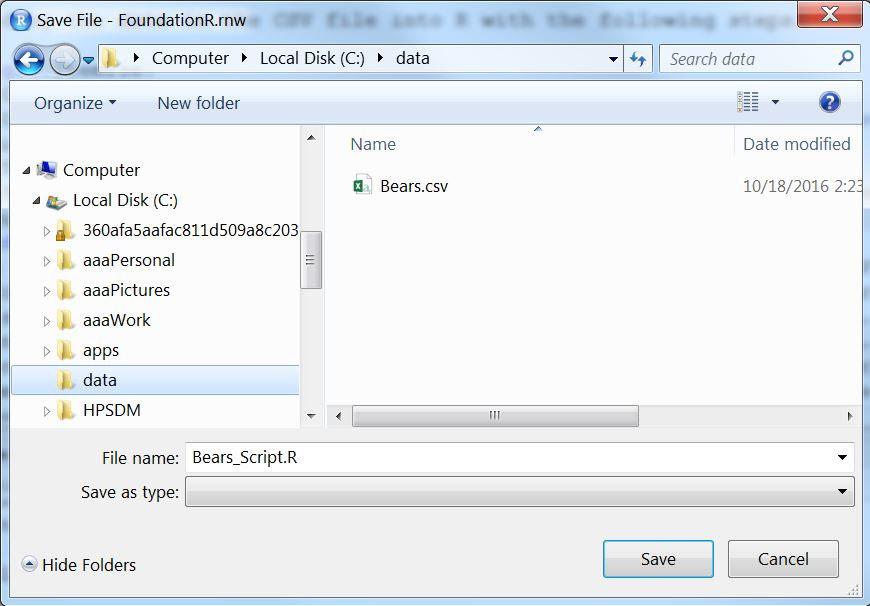
\includegraphics[width=3.5in]{Figs/Data_File_3.jpg}
\end{center}

  \item Set the working directory (tell R where the file is) with the \verb"Session", \verb"Set Working Directory ...", \verb"To Source File Location" menu items in RStudio.  RStudio will print an appropriate \R{setwd()} command to the console.  Copy this command from the console to the second line in your script.\footnote{Doing this will eliminate the need to manually select the menu options every time you want to run this script.}  For example, I stored the file created above in the \verb"C:/data" directory, so that RStudio will create this \R{setwd("C:/data")}.
  \item The CSV file is read into R by including the name of the file (in quotes) in \R{read.csv()}.  For example, \R{"Bears.csv"} is read into R and stored into an object called \R{bears} with \R{bears <- read.csv("Bears.csv")}.


  \item One should check the data in this object as descried in \sectref{sect:RViewdf} below
\end{Itemize}

\warn{Data stored in an external CSV file is read into R with \R{read.csv()}.}

It is important that each row of the data.frame correspond to one individual.  This is critically important when data are recorded for two different groups (e.g., for a two-sample t-test; see \modref{chap:tTest2}).  For example, the following data are methyl mercury levels recorded in mussels from two locations labeled as ``impacted'' and ``reference.''
\begin{Verbatim}
  impacted   0.011  0.054  0.056  0.095  0.051  0.077
  reference  0.031  0.040  0.029  0.066  0.018  0.042  0.044
\end{Verbatim}
To follow the ``one individual per row'' rule, these data are entered in stacked format where the ``reference'' data are stacked underneath the ``impacted'' data and a column is used to indicate to which group the individuals belong.  For example, the Excel file for data entry would look like the following

\begin{center}
  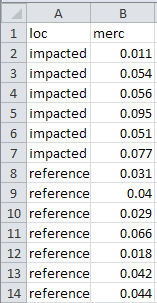
\includegraphics[width=1in]{Figs/StackedData.jpg}
\end{center}

\warn{Data files are constructed with data from only one individual in each row.}

\subsubsection*{Alternative Forms of Getting Data} \label{sect:RAltData}
\vspace{-12pt}
Some of the data files that you will use are provided on the \href{http://derekogle.com/NCMTH107/resources/data_107}{Data for MTH107} resource page of the class webpage.  In these cases, the data should be downloaded from the webpage and saved in the same directory or folder as your analysis script.  The downloaded file is then read into R in the same manner as described previously (i.e., set the working directory with \R{setwd()} and use \R{read.csv()}).

A few data files used in this book are supplied with R or the NCStats package.  These files are loaded with \R{data()}.  For example, the \dfile{iris} data file is loaded into R with
\begin{knitrout}
\definecolor{shadecolor}{rgb}{0.922, 0.922, 0.922}\color{fgcolor}\begin{kframe}
\begin{verbatim}
> data(iris)
\end{verbatim}
\end{kframe}
\end{knitrout}


\subsection{Working With Data Frames}  \label{sect:RWorkdf}
\vspace{-12pt}
\subsubsection{Viewing a Data Frame}  \label{sect:RViewdf}
\vspace{-12pt}
Many users are disoriented in RStudio because they cannot ``see'' their data in the same way that they see it in a spreadsheet program.  There are, however, several options for viewing your data.  First, you can type the name of the data.frame object to see its entire contents.
\begin{knitrout}
\definecolor{shadecolor}{rgb}{0.922, 0.922, 0.922}\color{fgcolor}\begin{kframe}
\begin{verbatim}
> bears
   length.cm weight.kg      loc
1      139.0       110 Bayfield
2      138.0        60 Bayfield
3      139.0        90 Bayfield
4      120.5        60 Bayfield
5      149.0        85 Bayfield
6      141.0       100  Ashland
7      141.0        95  Ashland
8      150.0        85  Douglas
9      166.0       155  Douglas
10     151.5       140  Douglas
11     129.5       105  Douglas
12     150.0       110  Douglas
\end{verbatim}
\end{kframe}
\end{knitrout}

Typing the name is adequate for small data.frames, but not useful for large data.frames.  The entire data.frame is opened in a separate window by double-clicking on the name of the data.frame in the \R{Environment} tab of RStudio.  Alternatively, the first and last three rows are viewed by including the data.frame object in \R{headtail()}.
\begin{knitrout}
\definecolor{shadecolor}{rgb}{0.922, 0.922, 0.922}\color{fgcolor}\begin{kframe}
\begin{verbatim}
> headtail(bears)
   length.cm weight.kg      loc
1      139.0       110 Bayfield
2      138.0        60 Bayfield
3      139.0        90 Bayfield
10     151.5       140  Douglas
11     129.5       105  Douglas
12     150.0       110  Douglas
\end{verbatim}
\end{kframe}
\end{knitrout}

In addition to viewing the contents, it is useful to examine the structure of the data.frame as returned from \R{str()}.  In this example, it is seen that three variables were recorded on 12 individuals.  The first variables -- \var{length.cm} and \var{weight.kg} -- are numerical measurements made on the bears.  The last variable -- \var{loc} -- is a factor variable that records the capture location for each bear.
\begin{knitrout}
\definecolor{shadecolor}{rgb}{0.922, 0.922, 0.922}\color{fgcolor}\begin{kframe}
\begin{verbatim}
> str(bears)
'data.frame':	12 obs. of  3 variables:
 $ length.cm: num  139 138 139 120 149 ...
 $ weight.kg: int  110 60 90 60 85 100 95 85 155 140 ...
 $ loc      : Factor w/ 3 levels "Ashland","Bayfield",..: 2 2 2 2 2 1 1 3 3 3 ...
\end{verbatim}
\end{kframe}
\end{knitrout}
The levels of the \var{loc} variable may be seen by including this variable (with the data.frame name) as the argument to \R{levels()}.
\begin{knitrout}
\definecolor{shadecolor}{rgb}{0.922, 0.922, 0.922}\color{fgcolor}\begin{kframe}
\begin{verbatim}
> levels(bears$loc)
[1] "Ashland"  "Bayfield" "Douglas" 
\end{verbatim}
\end{kframe}
\end{knitrout}

In the previous example, the \R{\$} notation was used to identify a particular variable (i.e., \R{loc}) within a data.frame (\R{bears}).  Think of variables as being nested inside data.frames and, thus, to access the variable you must first identify the data.frame in which it exists and then the name of the variable.  The \R{\$} simply separates the data.frame from the variable.
\begin{knitrout}
\definecolor{shadecolor}{rgb}{0.922, 0.922, 0.922}\color{fgcolor}\begin{kframe}
\begin{verbatim}
> bears$length.cm
 [1] 139.0 138.0 139.0 120.5 149.0 141.0 141.0 150.0 166.0 151.5 129.5 150.0
> bears$loc
 [1] Bayfield Bayfield Bayfield Bayfield Bayfield Ashland  Ashland  Douglas  Douglas 
[10] Douglas  Douglas  Douglas 
Levels: Ashland Bayfield Douglas
\end{verbatim}
\end{kframe}
\end{knitrout}

\warn{A dollar sign is ONLY used in R to separate the name of a data.frame from the name of a variable within that data.frame.}

\subsubsection{Selecting Individuals}  \label{sect:RSelectIndivs}
\vspace{-12pt}

In some instances, it may be important to select or exclude an individual from a data.frame.  Data.frames are two-dimensional objects that are indexed by a row and a column, in that order.  Positions within a data.frame are selected within paired square brackets.  For example, the item in the third row and second column of \R{bears} is selected below.
\begin{knitrout}
\definecolor{shadecolor}{rgb}{0.922, 0.922, 0.922}\color{fgcolor}\begin{kframe}
\begin{verbatim}
> bears[3,2]
[1] 90
\end{verbatim}
\end{kframe}
\end{knitrout}

\warn{Identifying the position of an item in an object is the ONLY time that square brackets are used in R.}

An entire row or column may be selected by omitting the other dimension.  For example, one could select the entire second column with \R{bears[,2]}, but this is also the \R{weight.kg} variable and is better selected, as shown above, with \R{bears\$weight.kg}.  As a better example, the entire third row is selected below (note that the column designation was omitted).
\begin{knitrout}
\definecolor{shadecolor}{rgb}{0.922, 0.922, 0.922}\color{fgcolor}\begin{kframe}
\begin{verbatim}
> bears[3,]
  length.cm weight.kg      loc
3       139        90 Bayfield
\end{verbatim}
\end{kframe}
\end{knitrout}

Multiple rows are selected by combining row indices together with \R{c()} (more about \R{c()} in \sectref{sect:RVectors}).  For example, the third, fifth, and eighth rows are selected below (again, the column index is omitted).
\begin{knitrout}
\definecolor{shadecolor}{rgb}{0.922, 0.922, 0.922}\color{fgcolor}\begin{kframe}
\begin{verbatim}
> bears[c(3,5,8),]
  length.cm weight.kg      loc
3       139        90 Bayfield
5       149        85 Bayfield
8       150        85  Douglas
\end{verbatim}
\end{kframe}
\end{knitrout}

Finally, rows can be excluded by preceding the row indices with a negative sign.
\begin{knitrout}
\definecolor{shadecolor}{rgb}{0.922, 0.922, 0.922}\color{fgcolor}\begin{kframe}
\begin{verbatim}
> bears[-c(3,5,8,10,12),]
   length.cm weight.kg      loc
1      139.0       110 Bayfield
2      138.0        60 Bayfield
4      120.5        60 Bayfield
6      141.0       100  Ashland
7      141.0        95  Ashland
9      166.0       155  Douglas
11     129.5       105  Douglas
\end{verbatim}
\end{kframe}
\end{knitrout}

\vspace{-12pt}
\subsubsection{Filtering a data.frame}  \label{sect:RSubsetdf}
\vspace{-12pt}
It is common to create a new data.frame that contains only some of the individuals from an existing data.frame.  For example, a researcher may want a data.frame of only bears captured in Bayfield County or bears that weighed more than 100 kg.  The process of creating the newer, smaller data.frame is called filtering (or subsetting) and is accomplished with \R{filterD()}.  The \R{filterD()} function requires the original data.frame as the first argument and a condition statement as the second argument.  The condition statement is used to either include or exclude individuals from the original data.frame.  Condition statements consist of the name of a variable in the original data.frame, a comparison operator, and a comparison value \tabrefp{tab:RSubsetConditions}.  The result from \R{filterD()} should be assigned to an object, which is then the name of the new data.frame.

\warn{\R{filterD()} is used to create a new data.frame that consists of individuals selected by some criterion from an existing data.frame.}

\begin{table}[htbp]
  \caption{Condition operators used in \R{filterD()} and their results.  Note that \emph{variable} generically represents a variable in the original data.frame and \emph{value} is a generic value or level.  Both \emph{variable} and \emph{value} would be replaced with specific items.}  \label{tab:RSubsetConditions}
  \centering
\begin{tabular}{cc}
\hline\hline
Condition Operator &  Individuals Returned from Original Data Frame \\
\hline
\widen{-1}{6}{\emph{variable}} $==$ \emph{value} & all individual that are \textbf{equal} to the given value \\
\widen{-1}{5}{\emph{variable}} $!=$ \emph{value} & all individuals that are \textbf{NOT equal} to the given value \\
\widen{-1}{5}{\emph{variable}} $>$ \emph{value} & all individuals that are \textbf{greater than} the given value \\
\widen{-1}{5}{\emph{variable}} $>=$ \emph{value} & all individuals that are \textbf{greater than or equal} to the given value \\
\widen{-1}{5}{\emph{variable}} $<$ \emph{value} & all individuals that are \textbf{less than} the given value \\
\widen{-1}{5}{\emph{variable}} $<=$ \emph{value} & all individuals that are \textbf{less than or equal} to the given value \\
\widen{-1}{5}{\emph{condition}}, \emph{condition} & all individuals that \textbf{meet both conditions} \\
\widen{-2}{6}{\emph{condition}} $|$ \emph{condition} & all individuals that \textbf{meet one or both conditions}\footnote{Note that this ``or'' operator is a ``vertical line'' which is typed with the shift-backslash key.} \\
\hline\hline
\end{tabular}
\end{table}

\vspace{18pt}
The following are examples of new data.frames created from \var{bears}.  The name of the new data.frame (i.e., object to the left of the assignment operator) can be any valid object name.  As demonstrated below, the new data.frame (or its structure) should be examined after each filtering to ensure that the data.frame actually contains the items that you desire.

\begin{itemize}
  \item Only individuals from \emph{Bayfield} county.
\begin{knitrout}
\definecolor{shadecolor}{rgb}{0.922, 0.922, 0.922}\color{fgcolor}\begin{kframe}
\begin{verbatim}
> bf <- filterD(bears,loc=="Bayfield")
> bf
  length.cm weight.kg      loc
1     139.0       110 Bayfield
2     138.0        60 Bayfield
3     139.0        90 Bayfield
4     120.5        60 Bayfield
5     149.0        85 Bayfield
\end{verbatim}
\end{kframe}
\end{knitrout}

  \item Individuals from both \emph{Bayfield} and \emph{Ashland} counties.
\begin{knitrout}
\definecolor{shadecolor}{rgb}{0.922, 0.922, 0.922}\color{fgcolor}\begin{kframe}
\begin{verbatim}
> bfash <- filterD(bears,loc %in% c("Bayfield","Ashland"))
> bfash
  length.cm weight.kg      loc
1     139.0       110 Bayfield
2     138.0        60 Bayfield
3     139.0        90 Bayfield
4     120.5        60 Bayfield
5     149.0        85 Bayfield
6     141.0       100  Ashland
7     141.0        95  Ashland
\end{verbatim}
\end{kframe}
\end{knitrout}

  \item Individuals with a weight greater than 100 kg.
\begin{knitrout}
\definecolor{shadecolor}{rgb}{0.922, 0.922, 0.922}\color{fgcolor}\begin{kframe}
\begin{verbatim}
> gt100 <- filterD(bears,weight.kg>100)
> gt100
  length.cm weight.kg      loc
1     139.0       110 Bayfield
2     166.0       155  Douglas
3     151.5       140  Douglas
4     129.5       105  Douglas
5     150.0       110  Douglas
\end{verbatim}
\end{kframe}
\end{knitrout}

  \item Individuals from \emph{Douglas} County that weigh at least 150 kg.
\begin{knitrout}
\definecolor{shadecolor}{rgb}{0.922, 0.922, 0.922}\color{fgcolor}\begin{kframe}
\begin{verbatim}
> do150 <- filterD(bears,loc=="Douglas",weight.kg>=150)
> do150
  length.cm weight.kg     loc
1       166       155 Douglas
\end{verbatim}
\end{kframe}
\end{knitrout}
\end{itemize}

\warn{View or ``structure'' the data.frame from \R{filterD()} to be sure that it contains data.}

\begin{exsection}
  \item \label{revex:BasicsDataFrame1} \rhw{} Two students at Seattle Community College made biometric measurements on 25 Douglas fir (\emph{Pseudotsuga menziesii}) trees in the lowlands of western Washington.  The variables recorded in the \href{https://raw.githubusercontent.com/droglenc/NCData/master/DougFirBiometrics.csv}{DougFirBiometrics.csv} file are a unique tree identifier (\var{tree}), the observer's name (\var{observer}; either ``Ingrid'' or ``Dylan''), the circumference at breast height (meters; \var{circ}), the height to the eye of the observer (meters; \var{eyeht}), the horizontal distance between observer and tree (meters; \var{horizdist}), the angle between observer and top of tree (degrees; \var{angle}), and the estimated height of tree (meters; \var{height}) using right-angle trigonometry. \ansref{ans:BasicsDataFrame1}
  \begin{Enumerate}
    \item Read this data file into an object called \R{DF}.
    \item Examine the structure of this data.frame.
    \item Show all measurements made on the third tree. [Do not do this manually; use R code.]
    \item Show all estimated tree heights.
    \item Show the estimated tree height for the fifth tree.
    \item Show all measurements for all trees measured by ``Ingrid''.  [HINT: use filtering.]
    \item Show all estimated tree heights for all trees measured by ``Dylan''.  [HINT: use filtering.]
    \item Show all measurements for tree heights less than 10 m.  [HINT: use filtering.]
    \item Show all measurements for tree heights greater than 10 m and circumference less than 1 m.  [HINT: use filtering.]
  \end{Enumerate}
\end{exsection}

\vspace{-12pt}
\subsection{Vectors}  \label{sect:RVectors}
\vspace{-12pt}

Data.frames are the primary structure in which to store real data.  However, much simpler situations that don't require a data.frame may arise.  In R, items of the same data type \sectrefp{sect:RDataTypes} are stored in a one-dimensional ``list'' called a \emph{vector}.  Vectors are usually displayed in one row (with many columns), but they may also be thought of as a single column (with many rows).  Items are entered into a vector with \R{c()}, where the individual arguments are specific numbers, characters, or logical values.\footnote{Note that \R{c} comes from the word ``concatenate.''}  Items for a vector of characters must be contained within paired quotes.
\begin{knitrout}
\definecolor{shadecolor}{rgb}{0.922, 0.922, 0.922}\color{fgcolor}\begin{kframe}
\begin{verbatim}
> ( v <- c(1,2,5) )
[1] 1 2 5
> ( y <- c("Iowa","Minnesota","Wisconsin") )
[1] "Iowa"      "Minnesota" "Wisconsin"
\end{verbatim}
\end{kframe}
\end{knitrout}

\defn{Vector}{A one-dimensional list of items of the same data type.  The primary information storage unit in R.}

Single variables from a data.frame are vectors.  Vectors that are not extracted from a data.frame will only be used in this course for very simple lists of items, usually as arguments in a function.
\begin{knitrout}
\definecolor{shadecolor}{rgb}{0.922, 0.922, 0.922}\color{fgcolor}\begin{kframe}
\begin{verbatim}
> bears$length.cm
 [1] 139.0 138.0 139.0 120.5 149.0 141.0 141.0 150.0 166.0 151.5 129.5 150.0
\end{verbatim}
\end{kframe}
\end{knitrout}

\warn{The columns of a data.frame are accessed with the name of the data.frame, a dollar sign, and then the name of the variable -- i.e., generically, \R{dataframe\$varname}.}


\begin{exsection}
  \item \label{revex:BasicsData1}\rhw{} Create a vector called \var{h} that contains nine heights of people. \ansref{ans:BasicsData1}
  \item \label{revex:BasicsData2}\rhw{} Create a vector called \var{w} that contains nine weights of people. \ansref{ans:BasicsData2}
  \item \label{revex:BasicsData3}\rhw{} Create a vector called \var{hc} that contains nine hair colors of people. \ansref{ans:BasicsData3}
  \item \label{revex:BasicsData4}\rhw{} Create a vector called \var{m} that contains nine logical values (=\R{TRUE} if male). \ansref{ans:BasicsData4}
  \item \label{revex:BasicsData5}\rhw{} Using the vectors from the previous questions,  \ansref{ans:BasicsData5}
  \begin{Enumerate}
    \item ... create the largest possible data.frame (use \R{data.frame()}).
    \item ... identify the height of the third individual of this data.frame.
    \item ... identify the hair color for the sixth individual of this data.frame.
  \end{Enumerate}
\end{exsection}

    \part{Exploratory Data Analysis}



\chapter[Summary One Quant Var]{Summaries for One Quantitative Variable)} \label{chap:UnivEDAQuant1}
\begin{ChapObj}{\boxwidth}
  \textbf{Objectives:}
  \begin{Enumerate}
    \item Calculate median, mean, and mode of a quantitative variable,
    \item Calculate IQR, standard deviation, and range of a quantitative variable,
    \item Construct a histogram for a quantitative variable, and
    \item Construct a boxplot for a quantitative variable,
  \end{Enumerate}
\end{ChapObj}

\minitoc
\vspace{48pt}

\lettrine{S}{ummarizing large quantities of data with} few graphical or numerical summaries makes it is easier to identify meaning from data (discussed in \modref{chap:WhyStatsImportant}). Numeric and graphical summaries specific to a single quantitative variable are described in this module. Interpretations from these numeric and graphical summaries are described in the next module.

Two data sets will be considered in this module when making calculations ``by hand'' (i.e., without using R). The first data set consists of the number of open pit mines in countries that have open pit mines \tabrefp{tab:MineData}.\footnote{These data were collected from \href{https://en.wikipedia.org/wiki/List_of_open-pit_mines}{this page}. See \sectref{sect:REnterData} for how to enter these data into R.} The second data set is Richter scale recordings for 15 major earthquakes \tabrefp{tab:EQData}. A third data set -- number of days of ice cover at ice gauge station 9004 in Lake Superior -- will be used to demonstrate calculations with R. These data are in \href{https://raw.githubusercontent.com/droglenc/NCData/master/LakeSuperiorIce.csv}{LakeSuperiorIce.csv} and are loaded into \R{LSI} below.\footnote{See \sectref{sect:RAltData} for a description of how to access these data. These data are originally from the \href{http://www.nsidc.org/}{National Snow and Ice Data Center}.}
\begin{knitrout}
\definecolor{shadecolor}{rgb}{0.922, 0.922, 0.922}\color{fgcolor}\begin{kframe}
\begin{verbatim}
> LSI <- read.csv("data/LakeSuperiorIce.csv")
\end{verbatim}
\end{kframe}
\end{knitrout}


% latex table generated in R 3.4.0 by xtable 1.8-2 package
% Sun May 21 17:06:49 2017
\begin{table}[ht]
\centering
\caption{Number of open pit mines in countries that have open pit mines.} 
\label{tab:MineData}
\begin{tabular}{rrrrrrrrrrrrr}
   \hline
2.0 & 11.0 & 4.0 & 1.0 & 15.0 & 12.0 & 1.0 & 1.0 & 3.0 & 2.0 & 2.0 & 1.0 & 1.0 \\ 
  1.0 & 1.0 & 2.0 & 4.0 & 1.0 & 4.0 & 2.0 & 4.0 & 2.0 & 1.0 & 4.0 & 11.0 & 1.0 \\ 
   \hline
\end{tabular}
\end{table}


% latex table generated in R 3.4.0 by xtable 1.8-2 package
% Sun May 21 17:06:49 2017
\begin{table}[ht]
\centering
\caption{Richter scale recordings for 15 major earthquakes.} 
\label{tab:EQData}
\begin{tabular}{rrrrrrrrrrrrrrr}
   \hline
5.5 & 6.3 & 6.5 & 6.5 & 6.8 & 6.8 & 6.9 & 7.1 & 7.3 & 7.3 & 7.7 & 7.7 & 7.7 & 7.8 & 8.1 \\ 
   \hline
\end{tabular}
\end{table}



\section{Numerical Summaries} \label{sec:quEDACenter}
A ``typical'' value and the ``variability'' of a quantitative variable are often described from numerical summaries. Calculation of these summaries is described in this module, whereas their interpretation is described in \modref{chap:UnivEDAQuant1}. As you will see in \modref{chap:UnivEDAQuant1}, ``typical'' values are measures of \textbf{center} and ``variability'' is often described as \textbf{dispersion} (or spread). Three measures of center are the median, mean, and mode. Three measures of dispersion are the inter-quartile range, standard deviation, and range.

All measures computed in this module are summary statistics -- i.e., they are computed from individuals in a sample. Thus, the name of each measure should be preceded by ``sample'' -- e.g., sample median, sample mean, and sample standard deviation. These measures could be computed from every individual, if the population was known. These values would then be parameters and would be preceded by ``population'' -- e.g., population median, population mean, and population standard deviation.\footnote{See \modref{sect:IVPPSS} for clarification on the differences between populations and samples and parameters and statistics.}


\subsection{Median} \label{sec:Median}
The median is the value of the individual in the position that splits the \textbf{ordered} list of individuals into two equal-\textbf{sized} halves. In other words, if the data are ordered, half the values will be smaller than the median and half will be larger.

The process for finding the median consists of three steps,\footnote{Most computer programs use a more sophisticated algorithm for computing the median and, thus, will produce different results than what will result from applying these steps.}
\vspace{-8pt}
\begin{Enumerate}
  \item Order the data from smallest to largest.
  \item Find the ``middle \textbf{position}'' ($mp$) with $mp=\frac{n+1}{2}$.
  \item If $mp$ is an integer (i.e., no decimal), then the median is the value of the individual in that position. If $mp$ is not an integer, then the median is the average of the value immediately below and the value immediately above the $mp$.
\end{Enumerate}

As an example, the open pit data from \tabref{tab:MineData} are,

% latex table generated in R 3.4.0 by xtable 1.8-2 package
% Sun May 21 17:06:49 2017
\begin{tabular}{rrrrrrrrrrrrr}
  1 & 1 & 1 & 1 & 1 & 1 & 1 & 1 & 1 & 1 & 2 & 2 & 2 \\ 
  2 & 2 & 2 & 3 & 4 & 4 & 4 & 4 & 4 & 11 & 11 & 12 & 15 \\ 
  \end{tabular}


Because $n=26$, the $mp=\frac{26+1}{2}=13.5$. The $mp$ is not an integer so the median is the average of the values in the 13th and 14th ordered positions (i.e., the two positions closest to $mp$). Thus, the median number of open pit mines in this sample of countries is $\frac{2+2}{2}=2$.

Consider finding the median of the Richter Scale magnitude recorded for fifteen major earthquakes as another example (ordered data are in \tabref{tab:EQData}). Because $n=15$, the $mp=\frac{15+1}{2}=8$. The $mp$ is an integer so the median is the value of the individual in the 8th ordered position, which is 7.1.

\warn{Don't forget to order the data when computing the median.}


\subsection{Inter-Quartile Range}
Quartiles are the values for the three individuals that divide ordered data into four (approximately) equal parts. Finding the three quartiles consists of finding the median, splitting the data into two equal parts at the median, and then finding the medians of the two halves.\footnote{You should review how a median is computed before proceeding with this section.}  A concern in this process is that the median is NOT part of either half if there is an odd number of individuals. These steps are summarized as,
\begin{Enumerate}
  \item Order the data from smallest to largest.
  \item Find the median -- this is the second quartile (Q2).
  \item Split the data into two halves at the median. If $n$ is odd (so that the median is one of the observed values), then the median is not part of either half.\footnote{Some authors put the median into both halves when $n$ is odd. The difference between the two methods is minimal for large $n$.}
  \item Find the median of the lower half of data -- this is the 1st quartile (Q1).
  \item Find the median of the upper half of data -- this is the third quartile (Q3).
\end{Enumerate}

These calculations are illustrated with the open pit mine data (the median was computed in \sectref{sec:Median}). Because $n=26$ is even, the halves of the data split naturally into two halves each with 13 individuals. Therefore, the $mp=\frac{13+1}{2}=7$ and the median of each half is the value of the individual in the seventh position. Thus, $Q1=1$ and $Q3=4$.

% latex table generated in R 3.4.0 by xtable 1.8-2 package
% Sun May 21 17:06:49 2017
\begin{tabular}{rrrrrrr}
  1 & 1 & 1 & 1 & 1 & 1 & 1 \\ 
  1 & 1 & 1 & 2 & 2 & 2 &  \\ 
  2 & 2 & 2 & 3 & 4 & 4 & 4 \\ 
  4 & 4 & 11 & 11 & 12 & 15 &  \\ 
  \end{tabular}


In summary, the first, second, and third quartiles for the open pit mine data are 1, 2, and 4, respectively. These three values separate the ordered individuals into approximately four equally-sized groups -- those with values less than (or equal to) 1, with values between (inclusive) 1 and 2, with values between (inclusive) 2 and 4, and with values greater (or equal to) than 4.

As another example, consider finding the quartiles for the earthquake data \tabrefp{tab:EQData}. Recall from above \sectrefp{sec:Median} that the median (=7.1) is in the eighth position of the ordered data. The value in the eighth position will not be included in either half. Thus, the two halves of the data are 5.5, 6.3, 6.5, 6.5, 6.8, 6.8, 6.9 and 7.3, 7.3, 7.7, 7.7, 7.7, 7.8, 8.1. The middle position for each half is then $mp=\frac{7+1}{2}=4$. Thus, the median for each half is the individual in the fourth position. Therefore, the median of the first half is $Q1=6.5$ and the median of the second half is $Q3=7.7$.

The interquartile range (IQR) is the difference between $Q3$ and $Q1$, namely $Q3-Q1$. However, the IQR (as strictly defined) suffers from a lack of information. For example, what does an IQR of 9 mean?  It can have a completely different interpretation if the IQR is from values of 1 to 10 or if it is from values of 1000 to 1009. Thus, the IQR is more useful if presented as both $Q3$ and $Q1$, rather than as the difference. Thus, for example, the IQR for the open pit mine data is from a $Q3$ of 4 to a $Q1$ of 1 and the IQR for the earthquake data is from a $Q3$ of 7 to a $Q1$ of 6.5.

\warn{The IQR can be thought of as the ``range of the middle half of the data.''}

\vspace{-12pt}
\warn{When reporting the IQR, explicitly state both $Q3$ and $Q1$ (i.e., do not subtract them).}


\subsection{Mean}
The mean is the arithmetic average of the data. The sample mean is denoted by $\bar{x}$ and the population mean by $\mu$. The mean is simply computed by adding up all of the values and dividing by the number of individuals. If the measurement of the generic variable $x$ on the $i$th individual is denoted as $x_{i}$, then the sample mean is computed with these two steps,
\begin{Enumerate}
  \item Sum (i.e., add together) all of the values -- $\Sum_{i=1}^{n}x_{i}$.
  \item Divide by the number of individuals in the sample -- $n$.
\end{Enumerate}
or more succinctly summarized with this equation,

\begin{equation} \label{eqn:SampleMean}
     \bar{x} = \frac{\Sum_{i=1}^{n}x_{i}}{n}
\end{equation}

For example, the sample mean of the open pit mine data is computed as follows:

\[ \bar{x} = \frac{2+11+4+1+15+ ... +2+1+4+11+1}{26} = \frac{94}{26} = 3.6  \]

Note in this example with a discrete variable that it is possible (and reasonable) to present the mean with a decimal. For example, it is not possible for a country to have 3.6 open pit mines, but it IS possible for the mean of a sample of countries to be 3.6 open pit mines.

\warn{As a general rule-of-thumb, present the mean with one more decimal than the number of decimals it was recorded in.}



\subsection{Standard Deviation}\label{sect:StdDev}
The sample standard deviation, denoted by $s$, is computed with these six steps:
\begin{Enumerate}
  \item Compute the sample mean (i.e., $\bar{x}$).
  \item For each value ($x_{i}$), find the difference between the value and the mean (i.e., $x_{i}-\bar{x}$).
  \item Square each difference (i.e., $(x_{i}-\bar{x})^{2}$).
  \item Add together all the squared differences.
  \item Divide this sum by $n-1$. [\textit{Stopping here gives the sample variance, $s^{2}$.}]
  \item Square root the result from the previous step to get $s$.
\end{Enumerate}

These steps are neatly summarized with
\vspace{-6pt}
\begin{equation}
  \label{eqn:SampleSD}
     s = \sqrt{\frac{\Sum_{i=1}^{n}(x_{i}-\bar{x})^{2}}{n-1}}
\end{equation}

The calculation of the standard deviation of the earthquake data \tabrefp{tab:EQData} is facilitated with the calculations shown in \tabref{tab:SDCalc}. In \tabref{tab:SDCalc}, note that
\vspace{-6pt}
\begin{Itemize}
  \item $\bar{x}$ is the sum of the ``Value'' column divided by $n=15$ (i.e., $\bar{x}=7.07$).
  \item The ``Diff'' column is each observed value minus $\bar{x}$ (i.e., Step 2).
  \item The ``Diff$^2$'' column is the square of the differences (i.e., Step 3).
  \item The sum of the ``Diff$^2$'' column is Step 4.
  \item The sample variance (i.e., Step 5) is equal to this sum divided by $n-1=14$ or $\frac{6.773}{14}=0.484$.
  \item The sample standard deviation is the square root of the sample variance or $s=\sqrt{0.484}=0.696$.
\end{Itemize}

\begin{table}[htbp]
  \caption{Table showing an efficient calculation of the standard deviation of the earthquake data.}
  \label{tab:SDCalc}
    \centering
    \begin{tabular}{cccc}
\hline\hline
Indiv & Value & Diff & Diff$^2$ \\
i & $x_{i}$ & $x_{i}-\bar{x}$ & $(x_{i}-\bar{x})^{2}$ \\
\hline
1 & 5.5 & -1.57 & 2.454 \\
2 & 6.3 & -0.77 & 0.588 \\
3 & 6.5 & -0.57 & 0.321 \\
4 & 6.5 & -0.57 & 0.321 \\
5 & 6.8 & -0.27 & 0.071 \\
6 & 6.8 & -0.27 & 0.071 \\
7 & 6.9 & -0.17 & 0.028 \\
8 & 7.1 & 0.03 & 0.001 \\
9 & 7.3 & 0.23 & 0.054 \\
10 & 7.3 & 0.23 & 0.054 \\
11 & 7.7 & 0.63 & 0.401 \\
12 & 7.7 & 0.63 & 0.401 \\
13 & 7.7 & 0.63 & 0.401 \\
14 & 7,8 & 0.73 & 0.538 \\
15 & 8.1 & 1.03 & 1.068 \\
\hline
Sum & 106 & 0 & 6.773 \\
\hline\hline
    \end{tabular}
\end{table}

From this, on average, each earthquake is approximately 0.7 Richter Scale units different than the average earthquake in these data.

\warn{In the standard deviation calculations don't forget to take the square root of the variance.}

\vspace{-12pt}
\warn{The standard deviation is greater than or equal to zero.}

The standard deviation can be thought of as ``the average difference between the values and the mean.'' This is, however, not a strict definition because the formula for the standard deviation does not simply add the differences and divide by $n$ as this definition would imply. Notice in \tabref{tab:SDCalc} that the sum of the differences from the mean is 0. This will be the case for all standard deviation calculations using the correct mean, because the mean balances the distance to individuals below the mean with the distance of individuals above the mean (see \sectref{sect:MeanMedian} in the next module). Thus, the mean difference will always be zero. This ``problem'' is corrected by squaring the differences before summing them. To get back to the original units, the squaring is later ``reversed'' by the square root. So, more accurately, the standard deviation is the square root of the average squared differences between the values and the mean. Therefore, ``the average difference between the values and the mean'' works as a practical definition of the meaning of the standard deviation, but it is not strictly correct.

\warn{Use the fact that the sum of all differences from the mean equals zero as a check of your standard deviation calculation.}

Further note that the mean is the value that minimizes the value of the standard deviation calculation -- i.e., putting any other value besides the mean into the standard deviation equation will result in a larger value.

Finally, you may be wondering why the sum of the squared differences in the standard deviation calculation is divided by $n-1$, rather than $n$. Recall (from \sectref{sect:IVPPSS}) that statistics are meant to estimate parameters. The sample standard deviation is supposed to estimate the population standard deviation ($\sigma$). Theorists have shown that if we divide by $n$, $s$ will consistently underestimate $\sigma$. Thus, $s$ calculated in this way would be a biased estimator of $\sigma$. Theorists have found, though, that dividing by $n-1$ will cause $s$ to be an unbiased estimator of $\sigma$. Being unbiased is generally good -- it means that on average our statistic estimates our parameter (this concept is discussed in more detail in \modref{chap:SamplingDist}).


\subsection{Mode}
The mode is the value that occurs most often in a data set. For example, one open pit mine is the mode in the open pit mine data \tabrefp{tab:MCmode}.

% latex table generated in R 3.4.0 by xtable 1.8-2 package
% Sun May 21 17:06:49 2017
\begin{table}[ht]
\centering
\caption{Frequency of countries by each number of open pit mines.} 
\label{tab:MCmode}
\begin{tabular}{rrrrrrrr}
   \hline
Number of Mines & 1 & 2 & 3 & 4 & 11 & 12 & 15 \\ 
  Freq of Countries & 10 & 6 & 1 & 5 & 2 & 1 & 1 \\ 
   \hline
\end{tabular}
\end{table}


The mode for a continuous variable is the class or bin with the highest frequency of individuals. For example, if 0.5-unit class widths are used in the Richter scale data, then the modal class is 6.5-6.9 \tabrefp{tab:EQmode}.

% latex table generated in R 3.4.0 by xtable 1.8-2 package
% Sun May 21 17:06:49 2017
\begin{table}[ht]
\centering
\caption{Frequency of earthquakes by Richter Scale class.} 
\label{tab:EQmode}
\begin{tabular}{rllllll}
   \hline
Richter Scale Class & 5.5-5.9 & 6-6.4 & 6.5-6.9 & 7-7.4 & 7.5-7.9 & 8-8.4 \\ 
  Freq of Earthquakes & 1 & 1 & 5 & 3 & 4 & 1 \\ 
   \hline
\end{tabular}
\end{table}


Some data sets may have two values or classes with the maximum frequency. In these situations the variable is said to be \textbf{bimodal}.

\subsection{Range}
The range is the difference between the maximum and minimum values in the data and measures the ultimate dispersion or spread of the data. The range in the open pit mine data is 15-1 = 14.

The range should \textbf{never be used by itself} as a measure of dispersion. The range is extremely sensitive to outliers and is best used only to show all possible values present in the data. The range (as strictly defined) also suffers from a lack of information. For example, what does a range of 9 mean?  It can have a completely different interpretation if it came from values of 1 to 10 or if it came from values of 1000 to 1009. Thus, the range is more instructive if presented as both the maximum and minimum value rather than the difference.


\subsection{Computation of Summaries in R} \label{sect:DescStats}
All summary statistics described above, with the exception of the mode, is  calculated in R with \R{Summarize()}. To summarize a single variable a one-sided formula of the form \R{\TILDE quant} is used, where \R{quant} generically represents the quantitative variable, along with the \R{data=} argument. The number of digits after the decimal place is controlled with \R{digits=}.
\begin{knitrout}
\definecolor{shadecolor}{rgb}{0.922, 0.922, 0.922}\color{fgcolor}\begin{kframe}
\begin{verbatim}
> Summarize(~days,data=LSI,digits=2)
     n nvalid   mean     sd    min     Q1 median     Q3    max 
 42.00  39.00 107.85  21.59  48.00  97.00 114.00 118.00 146.00 
\end{verbatim}
\end{kframe}
\end{knitrout}

From this it is seen that the sample median is 114 days, sample mean is 107.8 days, sample IQR is from 97 to 118 days, the sample standard deviation is 21.59 days, and the range is from 48 to 146.



\newpage
\section{Graphical Summaries}
\subsection{Histogram}
A histogram plots the frequency of individuals (y-axis) in classes of values of the quantitative variable (x-axis). Construction of a histogram begins by creating classes of values for the variable of interest. The easiest way to create a list of classes is to divide the range (i.e., maximum minus minimum value) by a ``nice'' number near eight to ten, and then round up to make classes that are easy to work with. The ``nice'' number between eight and ten is chosen to make the division easy and will be the number of classes. For example, the range of values in the open pit mine example is 15-1 = 14. A ``nice'' value near eight and ten to divide this range by is seven. Thus, the classes should be two units wide (=14/7) and, for ease, will begin at 0 \tabrefp{tab:MineFreqTable}.

\vspace{-6pt}
\begin{table}[htbp]
  \caption{Frequency table of number of countries in two-mine-wide classes.}
  \label{tab:MineFreqTable}
    \begin{Verbatim}[xleftmargin=25mm]
Class      0-1   2-3   4-5   6-7   8-9 10-11 12-13 14-15
Frequency   10     7     5     0     0     2     1     1
    \end{Verbatim}
\end{table}
\vspace{-12pt}

The frequency of individuals in each class is then counted (shown in the second row of \tabref{tab:MineFreqTable}). The plot is prepared with values of the classes forming the x-axis and frequencies forming the y-axis (\figref{fig:MineHist1}A). The first bar added to this skeleton plot has the bottom-left corner at 0 and the bottom-right corner at 2 on the x-axis, and a height equal to the frequency of individuals in the 0 and 1 class (\figref{fig:MineHist1}B). A second bar is then added with the bottom-left corner at 2 and the bottom-right corner at 4 on the x-axis, and a height equal to the frequency of individuals in the 2 and 3 class (\figref{fig:MineHist1}C). This process is continued with the remaining classes until the full histogram is constructed (\figref{fig:MineHist1}D).

\begin{knitrout}
\definecolor{shadecolor}{rgb}{0.922, 0.922, 0.922}\color{fgcolor}\begin{figure}[hbtp]

{\centering \includegraphics[width=.6\linewidth]{Figs/MineHist1-1} 

}

\caption[Steps (described in text) illustrating the construction of a histogram]{Steps (described in text) illustrating the construction of a histogram.}\label{fig:MineHist1}
\end{figure}


\end{knitrout}

Ideally eight to ten classes are used in a histogram. Too many or too few bars make it difficult to identify the shape and may lead to different interpretations. A dramatic example of the effect of changing the number of classes is seen in histograms of the length of eruptions for the Old Faithful geyser \figrefp{fig:histOF}.

\begin{knitrout}
\definecolor{shadecolor}{rgb}{0.922, 0.922, 0.922}\color{fgcolor}


















































\begin{figure}[hbtp]

{\centering \animategraphics[width=.35\linewidth,controls,palindrome,autoplay]{1}{Figs/histOF-}{1}{52}

}

\caption[Histogram of length of eruptions for Old Faitfhul geyser with varying number of classes]{Histogram of length of eruptions for Old Faitfhul geyser with varying number of classes.}\label{fig:histOF}
\end{figure}


\end{knitrout}


\subsection{Boxplot}
The \textbf{five-number summary} consists of the minimum, Q1, median, Q3, and maximum values (effectively contains the range, IQR, and median). For example, the five-number summary for the open pit mine data is 1, 1, 2, 4, and 15 (all values computed in the previous section). The five-number summary may be displayed as a \textbf{boxplot}. A traditional boxplot (\figref{fig:MineBoxplot}-Left) consists of a horizontal line at the median, horizontal lines at Q1 and Q3 that are connected with vertical lines to form a box, and vertical lines from Q1 to the minimum and from Q3 to the maximum. In modern boxplots (\figref{fig:MineBoxplot}-Right) the upper line extends from Q3 to the last observed value that is within 1.5 IQRs of Q3 and the lower line extends from Q1 to the last observed value that is within 1.5 IQRs of Q1. Observed values outside of the whiskers are termed ``outliers'' by this algorithm and are typically plotted with circles or asterisks. If no individuals are deemed ``outliers'' by this algorithm, then the two traditional and modern boxplots will be the same.

\begin{knitrout}
\definecolor{shadecolor}{rgb}{0.922, 0.922, 0.922}\color{fgcolor}\begin{figure}[hbtp]

{\centering \includegraphics[width=.65\linewidth]{Figs/MineBoxplot-1} 

}

\caption[Traditional (Left) and modern (Right) boxplots of the open pit mine data]{Traditional (Left) and modern (Right) boxplots of the open pit mine data.}\label{fig:MineBoxplot}
\end{figure}


\end{knitrout}


\subsection{Construction of Graphs in R}
A simple (by default) histogram is constructed in R with \R{hist()} using a one-sided formula of the form \R{\TILDE quant}, where \R{quant} generically represents the quantitative variable, and the corresponding data frame in \R{data=}.\footnote{Note that this is the same formula used in \R{Summarize()}.} The x-axis label may be improved from the default value by including a label in \R{xlab=}. The width of the classes may be controlled with a positive integer in \R{w=}.\footnote{The endpoints for the classes may also be set by giving a vector of endpoints to \R{breaks=}.}

\begin{knitrout}
\definecolor{shadecolor}{rgb}{0.922, 0.922, 0.922}\color{fgcolor}\begin{kframe}
\begin{verbatim}
> hist(~days,data=LSI,xlab="Days of Ice Cover")      # Fig 5.4-Left
> hist(~days,data=LSI,xlab="Days of Ice Cover",w=20) # Fig 5.4-Right
\end{verbatim}
\end{kframe}\begin{figure}[hbtp]

{\centering 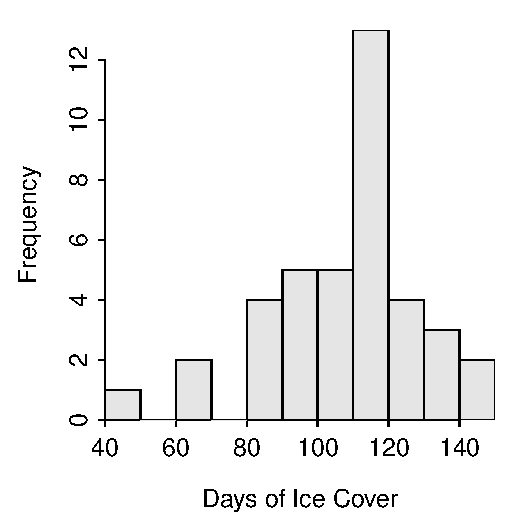
\includegraphics[width=.34\linewidth]{Figs/Histogram1-1} 
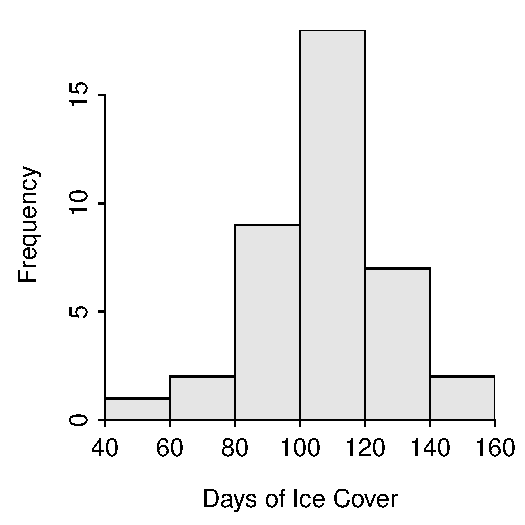
\includegraphics[width=.34\linewidth]{Figs/Histogram1-2} 

}

\caption[Histograms of the duration of ice cover at ice gauge 9004 in Lake Superior using the default class widths (Left) and widths of 20 days (Right)]{Histograms of the duration of ice cover at ice gauge 9004 in Lake Superior using the default class widths (Left) and widths of 20 days (Right).}\label{fig:Histogram1}
\end{figure}


\end{knitrout}

A modern boxplot of a single variable is constructed in R with \R{boxplot()}, where the first argument is usually a specific variable in a data.frame. Additionally, the y-axis may be properly labeled with \R{ylab=}.

\begin{knitrout}
\definecolor{shadecolor}{rgb}{0.922, 0.922, 0.922}\color{fgcolor}\begin{kframe}
\begin{verbatim}
> boxplot(LSI$days,ylab="Days of Ice Cover")
\end{verbatim}
\end{kframe}\begin{figure}[hbtp]

{\centering \includegraphics[width=.3\linewidth]{Figs/BoxplotLSI-1} 

}

\caption[Boxplot of the duration of ice cover at ice gauge 9004 in Lake Superior]{Boxplot of the duration of ice cover at ice gauge 9004 in Lake Superior.}\label{fig:BoxplotLSI}
\end{figure}


\end{knitrout}

\warn{The default histogram and boxplot should be modified by properly labeling the axes.}


\section{Multiple Groups} \label{sect:MultGroups}
It is common to need to compute numerical or construct graphical summaries of a quantitative variable separately for groups of individuals. In these cases it is beneficial to have a function that will efficiently construct a histogram and compute summary statistics for the quantitative variable separated by the levels of a factor variable. Separate histograms are constructed with \R{hist()}, if the first argument is a ``formula'' of the type \R{quant\TILDE group} where \R{quant} represents the quantitative response variable of interest and \R{group} represents the factor variable that indicates to which group the individual belongs. The data.frame that contains \R{quant} and \R{group} is given to \R{data=}. Summary statistics are separated by group by supplying the same formula and \R{data=} arguments to \R{Summarize()}.

As an example, the LSI data.frame contains a \R{period} variable that indicates whether the ice season was ``pre-1975'' or ``post-1975'' (which included 1975). Thus, one may be interested in examining the distribution of annual days of ice for each of these periods period. Histograms \figrefp{fig:mhist1} and summary statistics separated by period are constructed below.
\begin{knitrout}
\definecolor{shadecolor}{rgb}{0.922, 0.922, 0.922}\color{fgcolor}\begin{kframe}
\begin{verbatim}
> hist(days~period,data=LSI,ylab="Days of Ice Cover",w=20)
> Summarize(days~period,data=LSI,digits=2)
     period  n nvalid   mean    sd min Q1 median  Q3 max
1 post-1975 22     21 106.76 26.01  48 99  116.0 123 146
2  pre-1975 20     18 109.11 15.59  82 97  110.5 118 137
\end{verbatim}
\end{kframe}\begin{figure}[hbtp]

{\centering 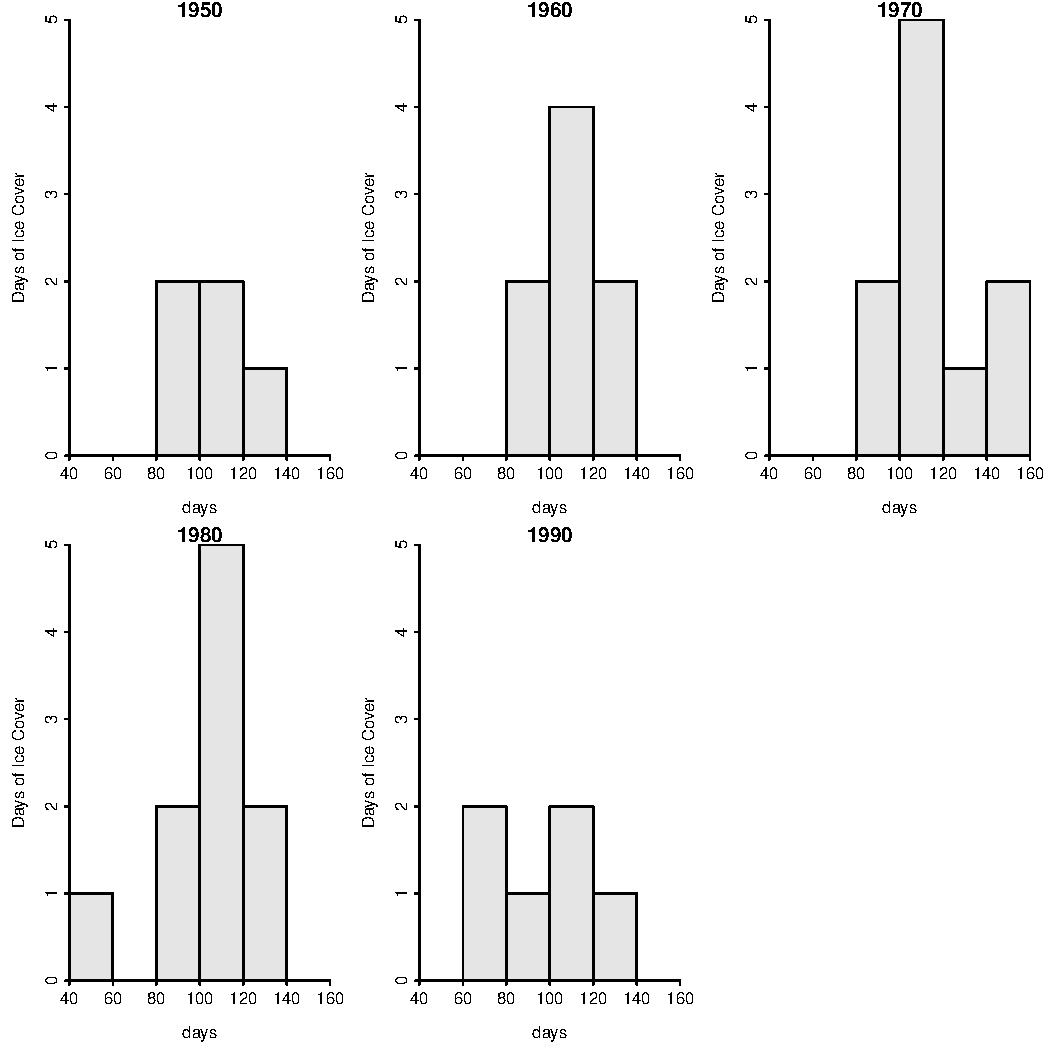
\includegraphics[width=.8\linewidth]{Figs/mhist1-1} 

}

\caption[Histograms of the duration of ice cover at ice gauge 9004 in Lake Superior by period]{Histograms of the duration of ice cover at ice gauge 9004 in Lake Superior by period.}\label{fig:mhist1}
\end{figure}


\end{knitrout}

Side-by-side boxplots \figrefp{fig:Boxplot1} are an alternative to separated histograms and are constructed by including the same formula and \R{data=} arguments to \R{boxplot()}.
\begin{knitrout}
\definecolor{shadecolor}{rgb}{0.922, 0.922, 0.922}\color{fgcolor}\begin{kframe}
\begin{verbatim}
> boxplot(days~period,data=LSI,ylab="Days of Ice Cover",xlab="Period")
\end{verbatim}
\end{kframe}\begin{figure}[hbtp]

{\centering 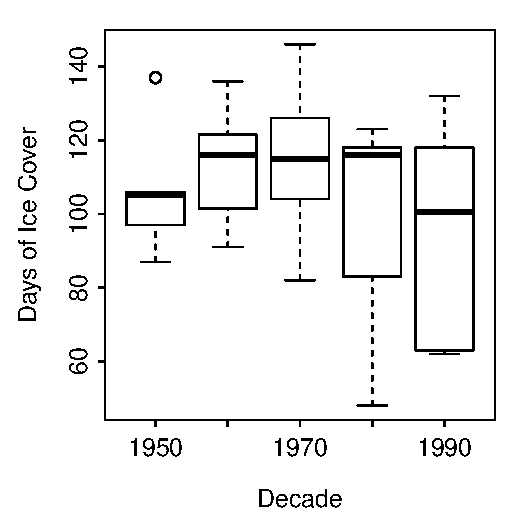
\includegraphics[width=.4\linewidth]{Figs/Boxplot1-1} 

}

\caption[Boxplot of the duration of ice cover at ice gauge 9004 in Lake Superior by period]{Boxplot of the duration of ice cover at ice gauge 9004 in Lake Superior by period.}\label{fig:Boxplot1}
\end{figure}


\end{knitrout}

Note that the formulae above required the grouping variable to be a factor. In some instances, a grouping variable may appear as an integer variable to R. For example, one may want to explore days of ice by decade, but the decade variable is not a factor variable.
\begin{knitrout}
\definecolor{shadecolor}{rgb}{0.922, 0.922, 0.922}\color{fgcolor}\begin{kframe}
\begin{verbatim}
> str(LSI)
'data.frame':	42 obs. of  5 variables:
 $ season: int  1955 1956 1957 1958 1959 1960 1961 1962 1963 1964 ...
 $ decade: int  1950 1950 1950 1950 1950 1960 1960 1960 1960 1960 ...
 $ period: Factor w/ 2 levels "post-1975","pre-1975": 2 2 2 2 2 2 2 2 2 2 ...
 $ temp  : num  22.9 23 25.7 20 24.8 ...
 $ days  : int  87 137 106 97 105 118 118 136 91 NA ...
\end{verbatim}
\end{kframe}
\end{knitrout}

In these cases, the variale needs to be explicitly converted to a factor variable using \R{factor()}, as shown below. The use of \R{factor()} is not needed if R already recognizes the variable as a factor variable.
\begin{knitrout}
\definecolor{shadecolor}{rgb}{0.922, 0.922, 0.922}\color{fgcolor}\begin{kframe}
\begin{verbatim}
> LSI$decade <- factor(LSI$decade)
> str(LSI)
'data.frame':	42 obs. of  5 variables:
 $ season: int  1955 1956 1957 1958 1959 1960 1961 1962 1963 1964 ...
 $ decade: Factor w/ 5 levels "1950","1960",..: 1 1 1 1 1 2 2 2 2 2 ...
 $ period: Factor w/ 2 levels "post-1975","pre-1975": 2 2 2 2 2 2 2 2 2 2 ...
 $ temp  : num  22.9 23 25.7 20 24.8 ...
 $ days  : int  87 137 106 97 105 118 118 136 91 NA ...
\end{verbatim}
\end{kframe}
\end{knitrout}



\chapter[Quant UnivEDA Interp]{Univariate EDA - Quantitative II (Interpretation)} \label{chap:UnivEDAQuant2}
\begin{ChapObj}{\boxwidth}
  \textbf{Objectives:}
  \begin{Enumerate}
    \item Use graphs to describe the shape of a distribution,
    \item Use graphs to describe outliers in a distribution,
    \item Identify which summary statistics are appropriate in a given situation, and
    \item Construct an appropriate overall summary.
  \end{Enumerate}
\end{ChapObj}

\minitoc
\newpage

\lettrine{M}{ethods for constructing numerical and graphical summaries} of a single quantitative variable were discussed in \modref{chap:UnivEDAQuant1}. Those summaries are interpreted here to provide an overall description of the distribution of the quantitative variable

\section{Items to Describe}
A univariate EDA for a quantitative variable is concerned with describing the distribution of the values for that variable; i.e., describing what values occurred and how often those values occurred.\index{EDA!Univariate!Quantitative}  Specifically, the distribution is described by four specific attributes:

\vspace{-12pt}
\begin{Enumerate}
  \item \textbf{shape} of the distribution,
  \item presence of \textbf{outliers},
  \item \textbf{center} of the distribution, and
  \item \textbf{dispersion} or spread of the distribution.
\end{Enumerate}
\vspace{-8pt}

Graphs are used to identify shape and the presence of outliers and to get a general feel for center and dispersion. However, numerical summaries are used to specifically describe center and dispersion of the data.

\vspace{-6pt}
\warn{Shape, center, dispersion, and outliers are described for each quantitative variable.}

\vspace{-12pt}
\warn{Shape and outliers are described from graphs; center and dispersion are describe with numerical summaries.}

The same three data sets used in \modref{chap:UnivEDAQuant1} are used here.

\vspace{-12pt}
\begin{Itemize}
  \item Measurements of water consumption in one hour by mice \tabrefp{tab:MouseData}.
  \item Richter scale recordings for 15 major earthquakes \tabrefp{tab:EQData}.
  \item The number of days of ice cover at ice gauge station 9004 in Lake Superior.
\end{Itemize}

\section{Interpreting Shape}\index{Histogram!Interpretation}
A histogram has two tails -- a left-tail for smaller or more negative values and a right-tail for larger or more positive values. The relative appearance of these two tails is used to identify three different shapes of distributions -- symmetric, left-skewed, and right-skewed.\index{Shape}\index{Symmetric}\index{Skewed}  If the left- and right-tail of a histogram are equal in shape (length and height), then the distribution is said to be \textbf{symmetric}. Perfectly symmetric distributions rarely occur in ``real-life.''  Therefore, if the left- and right-tail are approximately equal in shape, then the distribution is \textbf{approximately symmetric}. If the left-tail of the histogram is stretched out or, alternatively, the left-tail is longer and flatter than the right-tail, then the distribution is negatively- or \textbf{left-skewed}. If the right-tail of the histogram is stretched out or, alternatively, the right-tail is longer and flatter than the left-tail, then the distribution is positively- or \textbf{right-skewed}. The type of skew is defined by the longer tail; a longer right-tail means the distribution is right-skewed and a longer left-tail means it is left-skewed. Examples of each shape are shown in \figref{fig:ShapeExamples}.

\begin{knitrout}
\definecolor{shadecolor}{rgb}{0.922, 0.922, 0.922}\color{fgcolor}\begin{figure}[hbtp]

{\centering 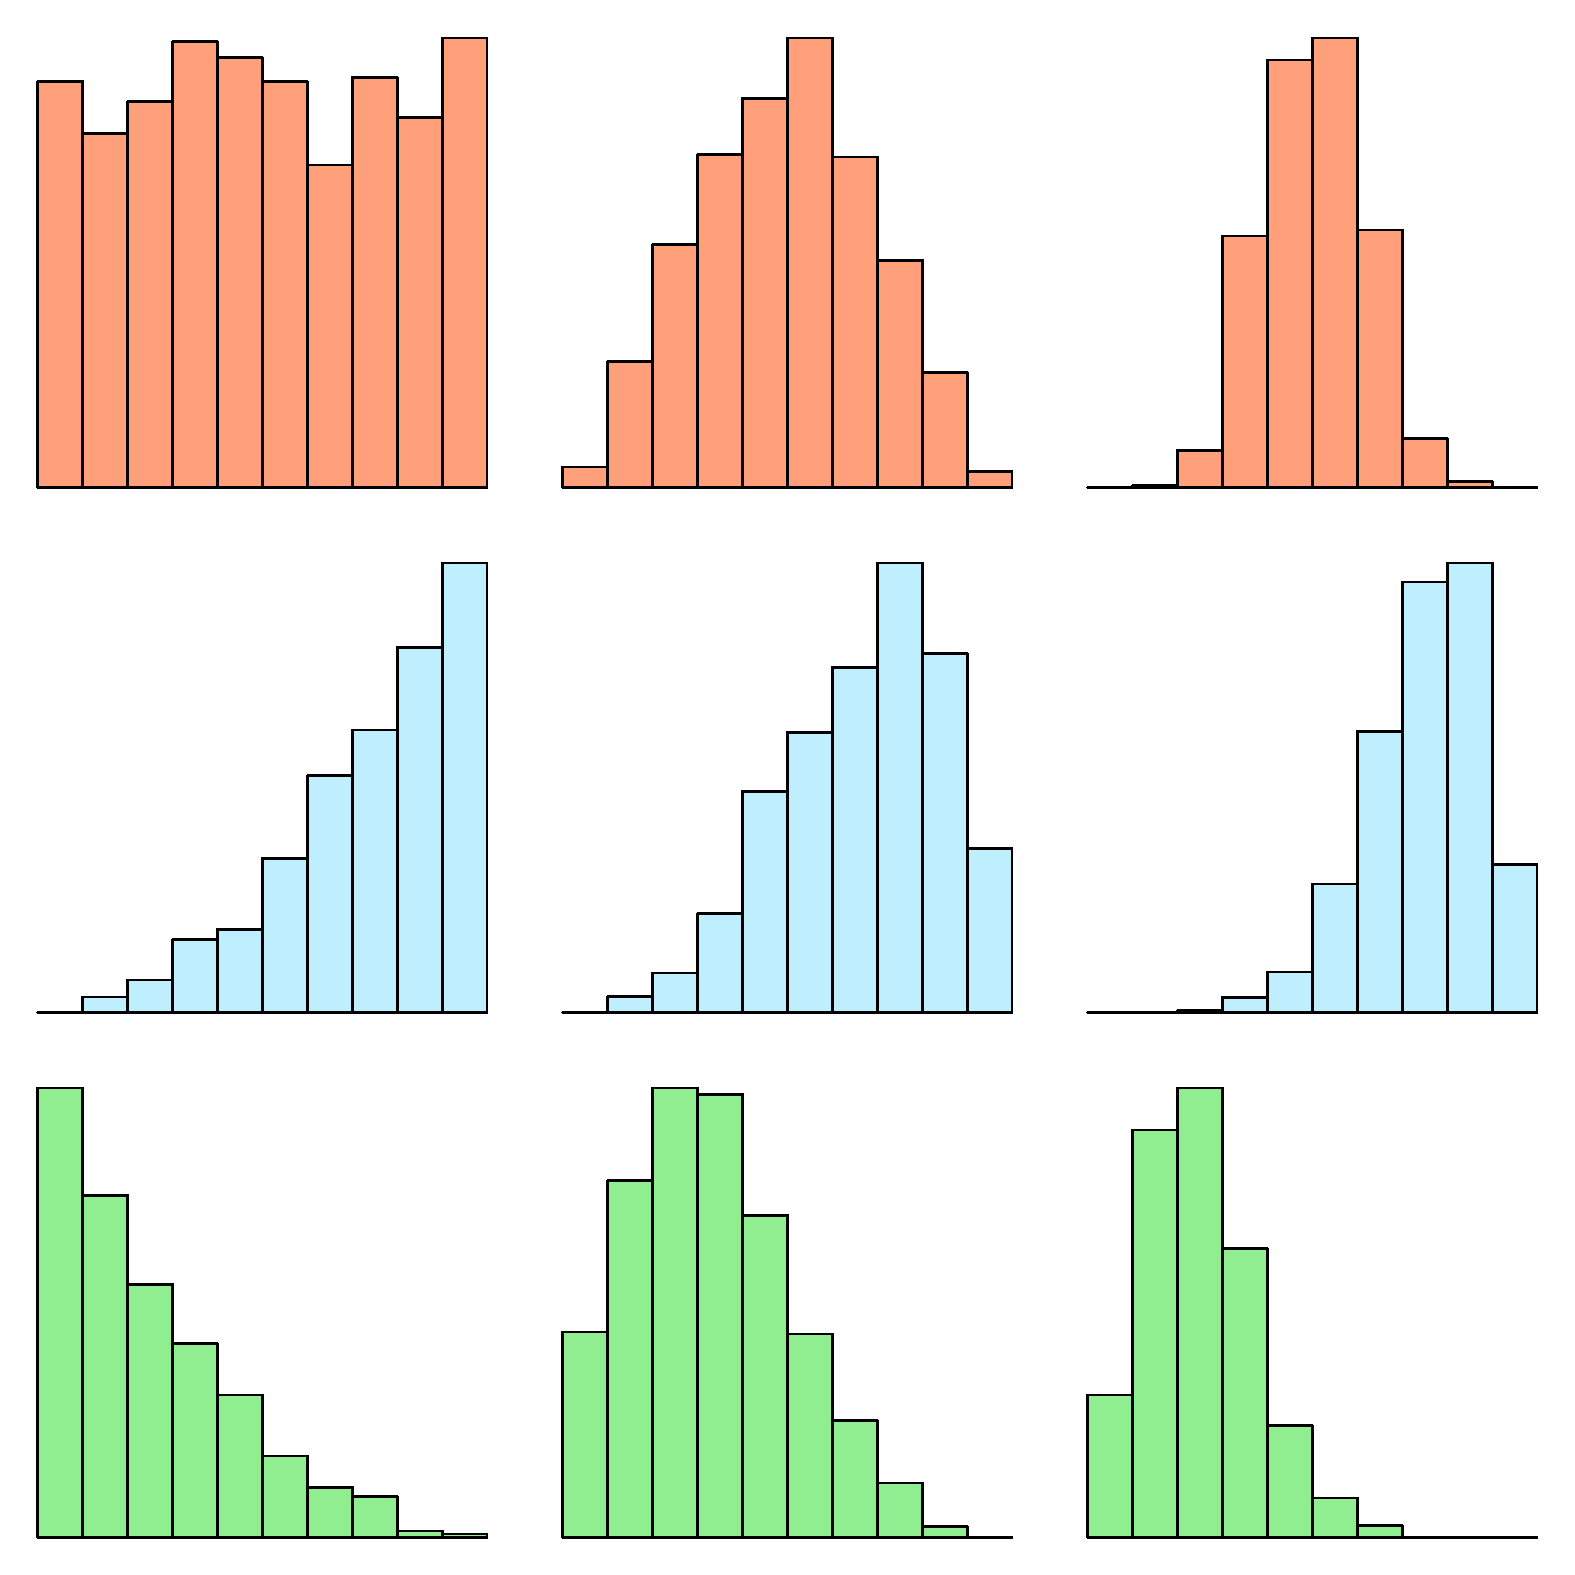
\includegraphics[width=.7\linewidth]{Figs/ShapeExamples-1} 

}

\caption[Examples of approximately symmetric (top, red), left-skewed (middle, blue), and right-skewed (bottom, green) histograms]{Examples of approximately symmetric (top, red), left-skewed (middle, blue), and right-skewed (bottom, green) histograms. Note that the axes labels were removed to focus attention on the shape of the histograms. Each histogram was constructed from n=1000 individuals and the x-axis range is from 0 to 1.}\label{fig:ShapeExamples}
\end{figure}


\end{knitrout}

\defn{Symmetric}{The left- and right-tail of a distribution are nearly the same in length and height.}

\vspace{-12pt}
\defn{Left-skewed}{The left-tail of a distribution is longer or more drawn out than the right-tail.}

\vspace{-12pt}
\defn{Right-skewed}{The right-tail of a distribution is longer or more drawn out than the left-tail.}

\vspace{-12pt}
\warn{The longer tail defines the type of skew.}

In practice, these labels form a continuum. For example, a perfectly symmetric distribution is rare. However, in the many cases of an asymmetric distribution, it is a fine line between calling the shape approximately symmetric or one of the skewed distributions.

\vspace{-12pt}
\warn{Symmetric, left-skewed, and right-skewed descriptors are guides; many ``real'' distributions will not fall neatly into these categories.}

The relative length from the median to Q1 and the median to Q3 (i.e., the position of the median line in the box) indicates the shape of the distribution.\index{Boxplot!Interpretation}  If the distribution is left-skewed (i.e., lesser-valued individuals are ``spread out''; \figref{fig:BoxplotShape}-Right), then median-Q1 will be greater than Q3-median. In contrast, if the distribution is right-skewed (i.e., larger-valued individuals are spread out; \figref{fig:BoxplotShape}-Middle), then Q3-median will be greater than median-Q1. Thus, if the distribution is right-skewed then the median will be closer to Q1 than to Q3, if the distribution is left-skewed then the median will be closer to Q3 than to Q1, and if the distribution is approximately symmetric (\figref{fig:BoxplotShape}-Left) then the median will be in the middle of the box.

\begin{knitrout}
\definecolor{shadecolor}{rgb}{0.922, 0.922, 0.922}\color{fgcolor}\begin{figure}[hbtp]

{\centering 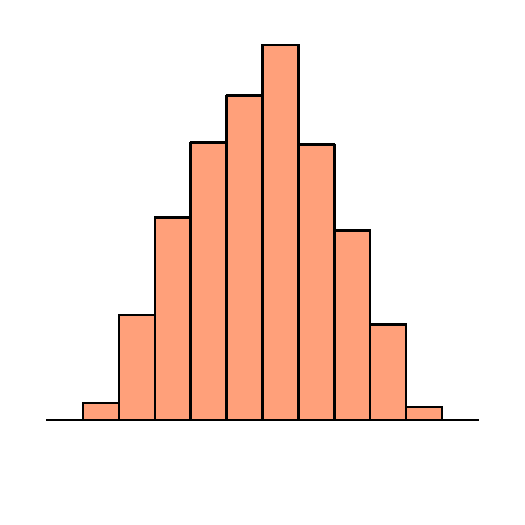
\includegraphics[width=.3\linewidth]{Figs/BoxplotShape-1} 
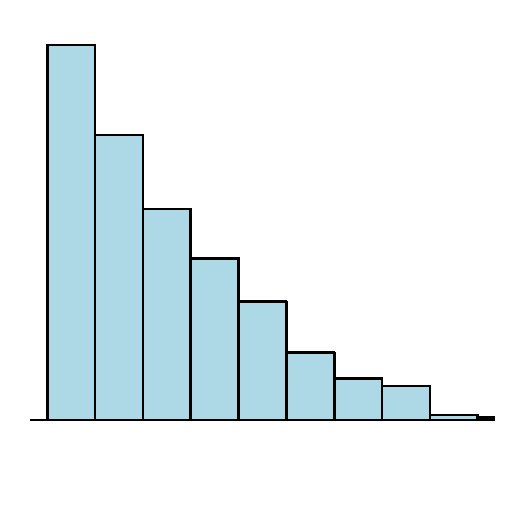
\includegraphics[width=.3\linewidth]{Figs/BoxplotShape-2} 
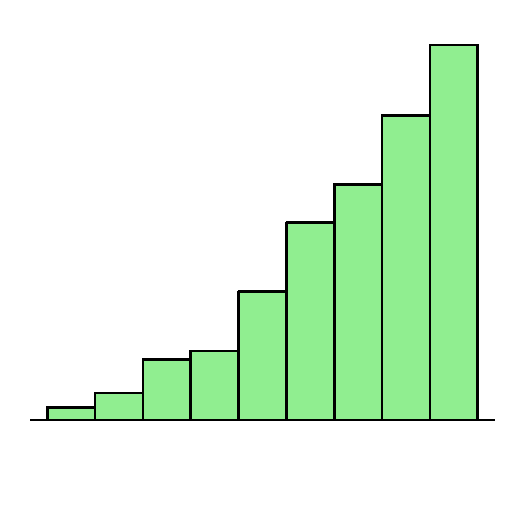
\includegraphics[width=.3\linewidth]{Figs/BoxplotShape-3} 
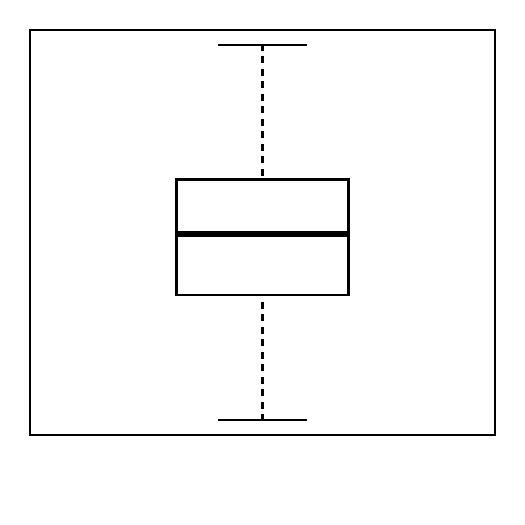
\includegraphics[width=.3\linewidth]{Figs/BoxplotShape-4} 
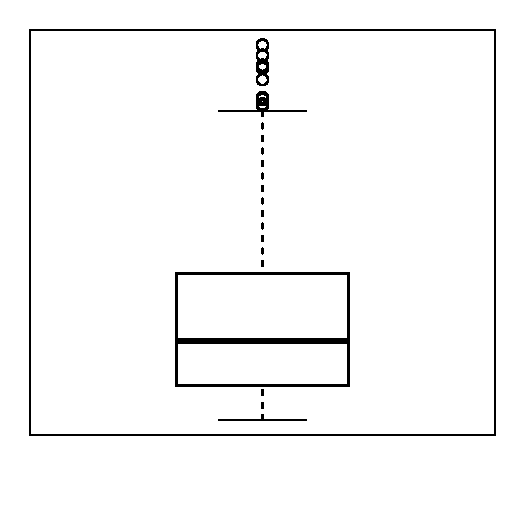
\includegraphics[width=.3\linewidth]{Figs/BoxplotShape-5} 
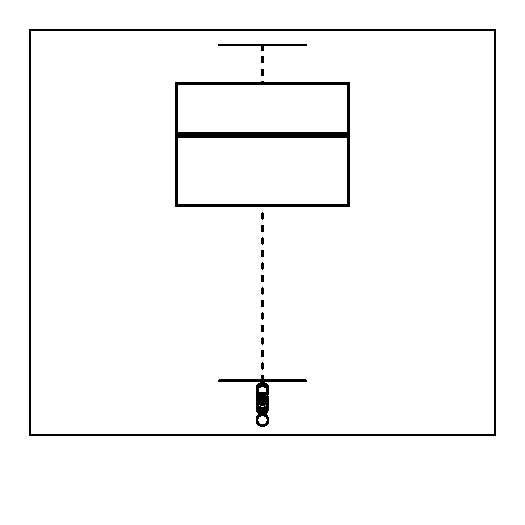
\includegraphics[width=.3\linewidth]{Figs/BoxplotShape-6} 

}

\caption[Histograms and boxplots for several different shapes of distributions]{Histograms and boxplots for several different shapes of distributions.}\label{fig:BoxplotShape}
\end{figure}


\end{knitrout}

\warn{If a distribution is right-skewed, then the median will be closer to Q1 than to Q3. If the distribution is left-skewed, then the median will be closer to Q3 than to Q1.}

\vspace{-12pt}
\warn{Even though shape can be described from a boxplot, it is always easier to describe shape from a histogram.}

\begin{exsection}
  \item \label{revex:quEDABrule5N} What is the five-number summary for the maximum gauge heights of the Bois Brule River in Brule, WI from Exercise \ref{revex:quEDABrule}. \ansref{ans:quEDABrule5N}
  \item \label{revex:quEDAWI5N} \rhw{} Construct a boxplot for the population density of Wisconsin counties from Exercise \ref{revex:quEDAWIc}. \ansref{ans:quEDAWI5N}
  \item \label{revex:quEDABoxLeft} What is the shape of the left boxplot below? \ansref{ans:quEDABoxLeft}

\begin{center}
  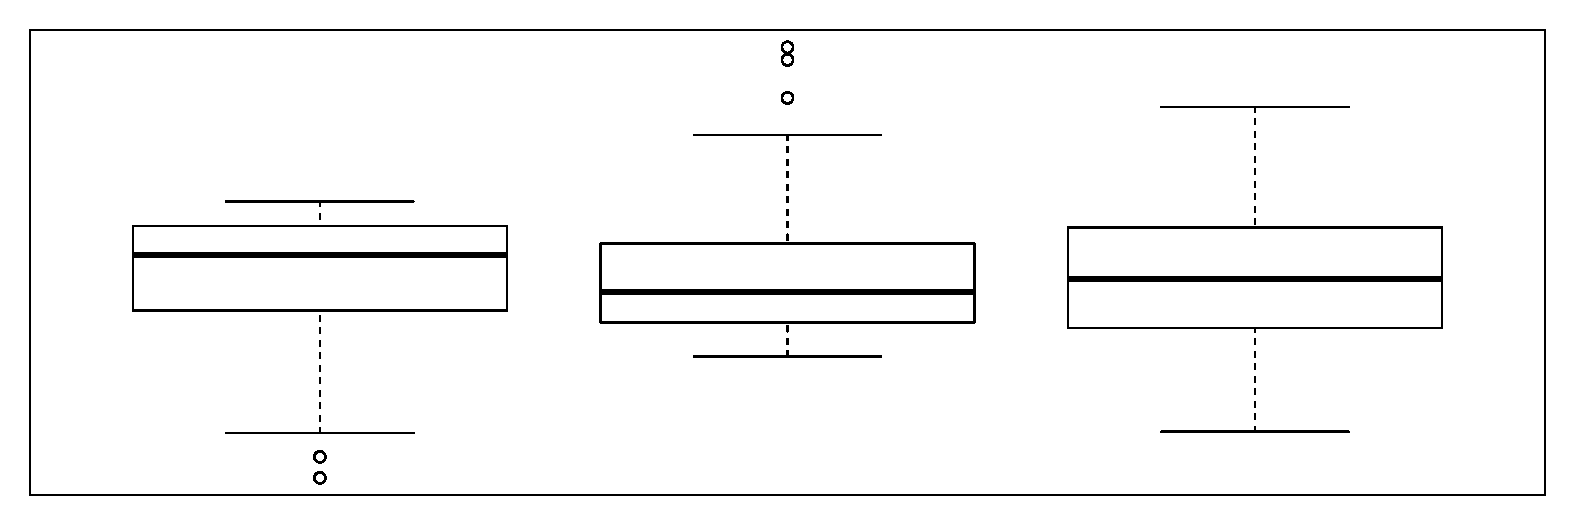
\includegraphics[width=4in]{Figs/BoxplotQuest-1}
\end{center}

  \item \label{revex:quEDABoxRight} What is the shape of the middle boxplot above? \ansref{ans:quEDABoxRight}
  \item \label{revex:quEDABoxSym} What is the shape of the right boxplot above? \ansref{ans:quEDABoxSym}
  \item \label{revex:quEDALSkewCtr} If the distribution is skewed left, which measure should you generally use to measure center? \ansref{ans:quEDALSkewCtr}
  \item \label{revex:quEDARSkewCtr} Which measure of center should you generally use for a right-skewed distribution? \ansref{ans:quEDARSkewCtr}
  \item \label{revex:quEDASymCtr} Which measure of center should you generally use for a symmetric distribution? \ansref{ans:quEDASymCtr}
  \item \label{revex:quEDASymDisp} Which measure of dispersion should you generally use for a symmetric distribution? \ansref{ans:quEDASymDisp}
  \item \label{revex:quEDALSkewDisp} Which measure of dispersion should you generally use for a left-skewed distribution? \ansref{ans:quEDALSkewDisp}
  \item \label{revex:quEDARSkewDisp} Which measure of dispersion should you generally use for a right-skewed distribution? \ansref{ans:quEDARSkewDisp}
  \item \label{revex:quEDAQShape1} Is Q3-Q2 less than, approximately equal to, or greater than Q2-Q1 if the data are left-skewed? \ansref{ans:quEDAQShape1}
  \item \label{revex:quEDAQShape2} What is the shape of the distribution if Q3-Q2 is greater than Q2-Q1? \ansref{ans:quEDAQShape2}
\end{exsection}


\section{Interpreting Outliers}\index{Outlier}\index{Histogram!Interpretation}
An outlier is an individual whose value is widely separated from the main cluster of values in the sample. On histograms, outliers appear as bars that are separated from the main cluster of bars by ``white space'' or areas with no bars \figrefp{fig:OutlierExHist}. In general, outliers must be on the margins of the histogram, should be separated by one or two missing bars, and should only be one or two individuals.

\begin{knitrout}
\definecolor{shadecolor}{rgb}{0.922, 0.922, 0.922}\color{fgcolor}\begin{figure}[hbtp]

{\centering 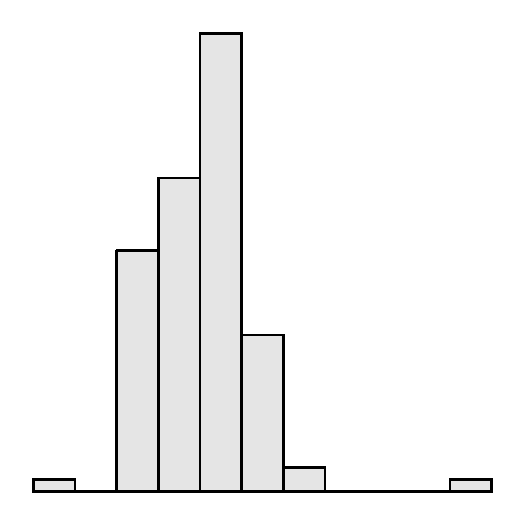
\includegraphics[width=.4\linewidth]{Figs/OutlierExHist-1} 

}

\caption[Example histogram with an outlier to the right]{Example histogram with an outlier to the right.}\label{fig:OutlierExHist}
\end{figure}


\end{knitrout}

\defn{Outlier}{An individual whose value is widely separated from the main cluster of values in the sample.}

An outlier may occur as a result of human error in the sampling process. If this is the case, then the value should be corrected or removed. Other times an outlier may be an individual that was not part of the population of interest -- e.g., an adult animal that was sampled when only immature animals were being considered. In this case, the individual's value should be removed from the sample. Still other times, an outlier is part of the population and should generally not be removed from the sample. In fact you may wish to highlight an outlier as an interesting observation! Regardless, it is important that you construct a histogram to determine if outliers are present or not.

Don't let outliers completely influence how you define the shape of a distribution. For example, if the main cluster of values is approximately symmetric and there is one outlier to the right of the main cluster (as illustrated in \figref{fig:OutlierExHist}), \textbf{DON'T} call the distribution right-skewed. You should describe this distribution as approximately symmetric with an outlier to the right.

\warn{Not all outliers warrant removal from your sample.}

\vspace{-12pt}
\warn{Don't let outliers completely influence how you define the shape of a distribution.}

\vspace{24pt}
\begin{exsection}
  \item \label{revex:quEDALSkew} What is a distribution with a long left-tail called? \ansref{ans:quEDALSkew}
  \item \label{revex:quEDARSkew} What is a distribution with a long right-tail called? \ansref{ans:quEDARSkew}
  \item \label{revex:quEDALSkewg} What is the shape of the distribution on the left below? \ansref{ans:quEDALSkewg}


\begin{center}
  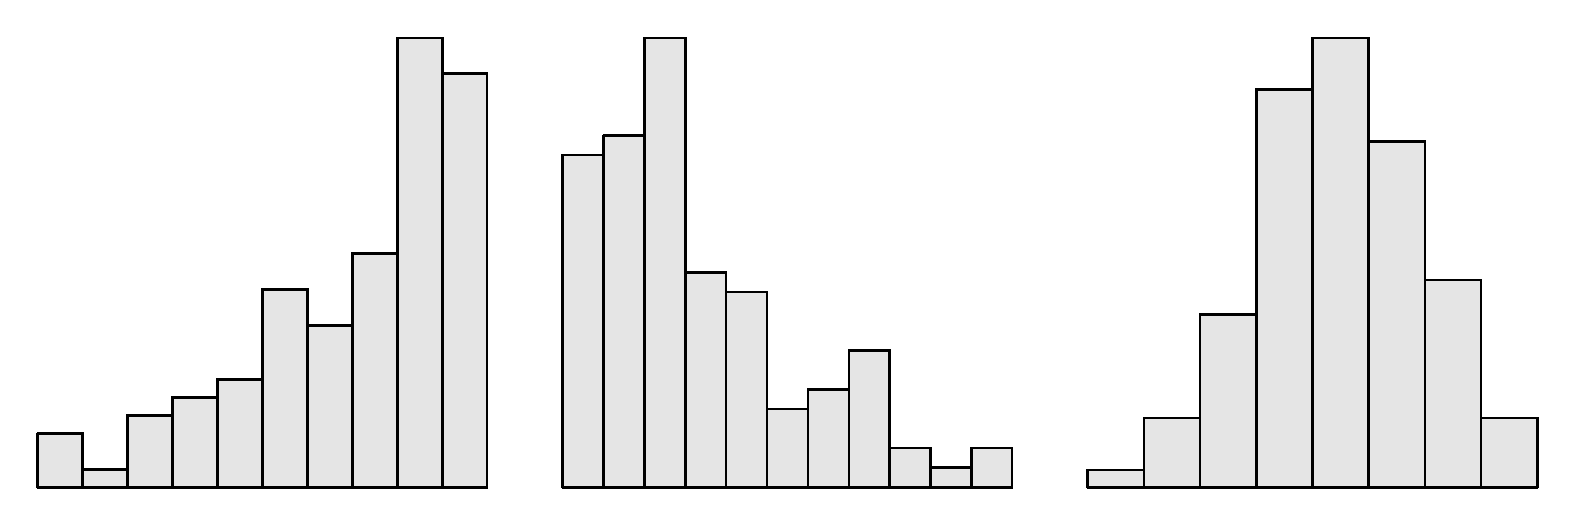
\includegraphics[width=5in]{Figs/HistQuest-1}
\end{center}
  \item \label{revex:quEDASymg} What is the shape of the distribution in the center above? \ansref{ans:quEDASymg}
  \item \label{revex:quEDARSkewg} What is the shape of the distribution on the right above? \ansref{ans:quEDARSkewg}
  \item \label{revex:quEDAlead} Comment on the shape and presence of outliers in \figref{fig:KreherParkPbhist}. \ansref{ans:quEDAlead}
\end{exsection}


\section{Comparing the Median and Mean} \label{sect:MeanMedian}
The mean and median measure center in different ways.\index{Median!Compared to mean}\index{Mean!Compared to median}\index{Mean!How measures center}\index{Median!How measures center}  The median is concerned with the \textbf{position} of the value rather than the value itself (recall how it is calculated). The mean, on the other hand, is the value such that the sum of the distances from it to all points smaller than it is the same as the sum of the distances from it to all points greater than it. The mean is very much concerned about the \textbf{values} for each individual, as the values are used to find the ``distance'' from the mean.

\warn{The actual values of the data (beyond ordering the data) are not considered when calculating the median; whereas the actual values are very much considered when calculating the mean.}

A plot of the Richter scale data against the corresponding ordered individual number is shown in \figref{fig:MeanMedianComp1}-Left.\footnote{This is a rather non-standard graph but it is useful for comparing how the mean and median measure the center of the data.}  The median (blue line) is found by locating the middle position on the individual number axis and then finding the corresponding Richter scale value (move right until the point is intercepted and then move down to the x-axis). The vertical blue line represents the median, and it can be seen that it has the same \textbf{number} of individuals (i.e., points) below it as above it. In contrast, the mean finds the Richter scale value that has the same total distance to values below it as total distance to values above it. In other words, the mean is the vertical red line so that the total \textbf{length} of the horizontal dashed red lines is the same to the left as it is to the right. Thus, the median balances the number of individuals above and below the median, whereas the mean balances the difference in values above and below the mean.

\begin{knitrout}
\definecolor{shadecolor}{rgb}{0.922, 0.922, 0.922}\color{fgcolor}\begin{figure}[hbtp]

{\centering 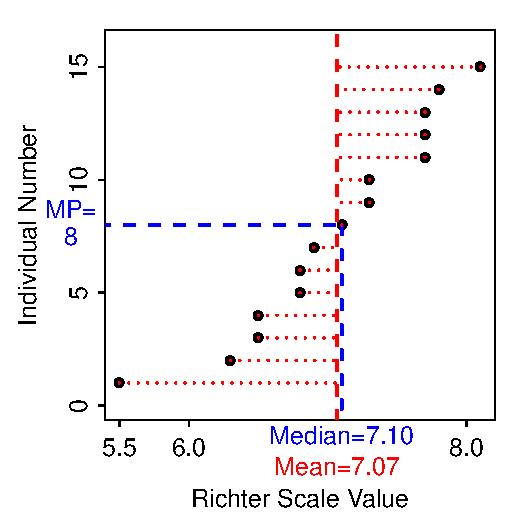
\includegraphics[width=.45\linewidth]{Figs/MeanMedianComp1-1} 
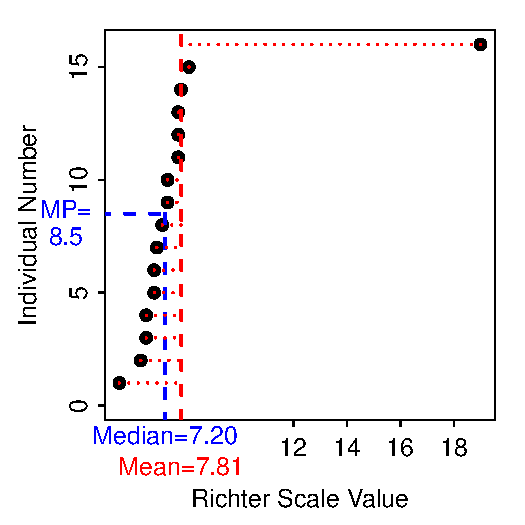
\includegraphics[width=.45\linewidth]{Figs/MeanMedianComp1-2} 

}

\caption[Plot of the individual number versus Richter scale values for the original earthquake data (\textbf{Left}) and the earthquake data with an extreme outlier (\textbf{Right})]{Plot of the individual number versus Richter scale values for the original earthquake data (\textbf{Left}) and the earthquake data with an extreme outlier (\textbf{Right}). The median value is shown as a blue vertical line and the mean value is shown as a red vertical line. Differences between each individual value and the mean value are shown with horizontal red lines.}\label{fig:MeanMedianComp1}
\end{figure}


\end{knitrout}

\warn{The mean balances the distance to individuals above and below the mean. The median balances the number of individuals above and below the median.}

\vspace{-12pt}
\warn{The sum of all differences between individual values and the mean (as properly calculated) equals zero.}

The mean and median differ in their sensitivity to outliers (\figref{fig:MeanMedianComp1}-Right).\index{Mean!Sensitivity to outliers}\index{Median!Sensitivity to outliers}  For example, suppose that an incredible earthquake with a Richter Scale value of 19.0 was added to the earthquake data set. With this additional individual, the median increases from 7.1 to 7.2, but the mean increases from 7.1 to 7.8. The outlier affects the value of the mean more than it affects the value of the median because of the way that each statistic measures center. The mean will be pulled towards an outlier because it must ``put'' many values on the ``side'' of the mean away from the outlier so that the sum of the differences to the larger values and the sum of the differences to the smaller values will be equal. Thus, the outlier in this example creates a large difference to the right of the mean so the mean has to ``move'' to the right to make this difference smaller, move more individuals to the left side of the mean, and increase the differences of individuals to the left of the mean to balance this one large individual. The median on the other hand will simply ``put'' one more individual on the side opposite of the outlier because it balances the number of individuals on each side of it. Thus, the median has to move very little to the right to accomplish this balance.

\warn{The mean is more sensitive (i.e., changes more) to outliers than the median; it will be ``pulled'' towards the outlier more than the median.}

The shape of the distribution, even if outliers are not present, also has an effect on the values of the mean and median as depicted in \figref{fig:MeanMedianShape}. If a distribution is perfectly symmetric, then the median and mean (along with the mode) will be identical. If the distribution is approximately symmetric, then the median and mean will be approximately equal. If the distribution is right-skewed, then the mean will be greater than the median. Finally, if the distribution is left-skewed, then the mean will be less than the median.

\begin{knitrout}
\definecolor{shadecolor}{rgb}{0.922, 0.922, 0.922}\color{fgcolor}\begin{figure}[hbtp]

{\centering 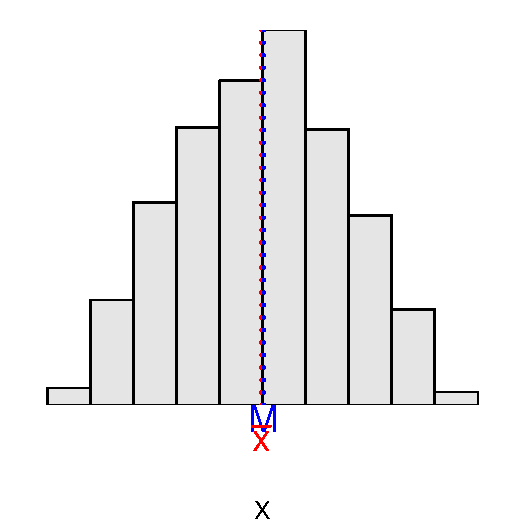
\includegraphics[width=.3\linewidth]{Figs/MeanMedianShape-1} 
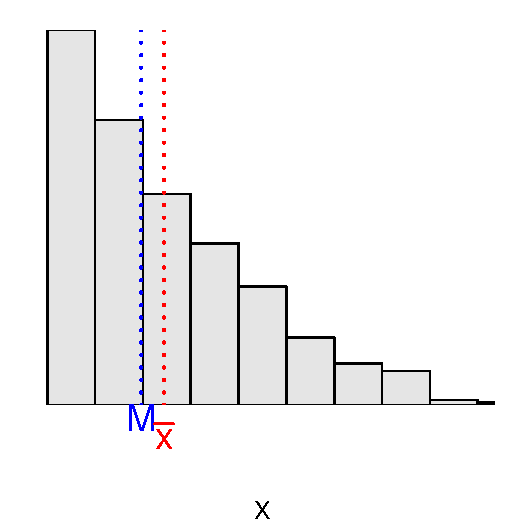
\includegraphics[width=.3\linewidth]{Figs/MeanMedianShape-2} 
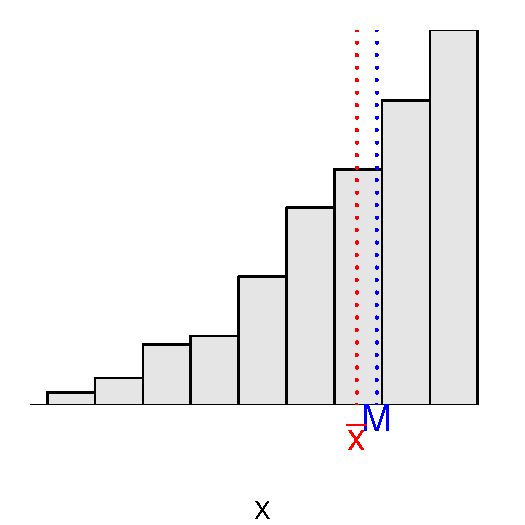
\includegraphics[width=.3\linewidth]{Figs/MeanMedianShape-3} 

}

\caption[Three differently shaped histograms with vertical lines superimposed at the median (M]{Three differently shaped histograms with vertical lines superimposed at the median (M; blue lines) and the mean ($\bar{x}$; red lines).}\label{fig:MeanMedianShape}
\end{figure}


\end{knitrout}

\warn{The mean and median are equal for symmetric distributions.}

\vspace{-12pt}
\warn{The mean is pulled towards the long tail of a skewed distribution. Thus, the mean is greater than the median for right-skewed distributions and the mean is less than the median for left-skewed distributions.}

As shown above, the mean and median measure center in different ways. The question now becomes ``which measure of center is better?''  The median is a ``better'' measure of center when outliers are present. In addition, the median gives a better measure of a typical individual when the data are skewed. Thus, in this course, the median is used when outliers are present or the distribution of the data is skewed.\index{Median!When to use}  If the distribution is symmetric, then the purpose of the analysis will dictate which measure of center is ``better.''  However, in this course, use the mean when the data are symmetric or, at least, not strongly skewed.\index{Mean!When to use}

\warn{Describe center with the median if outliers are present or the data are skewed; use the mean if the data are symmetric and no outliers are present.}

\vspace{-12pt}
\begin{exsection}
  \item \label{revex:quEDALSkewMM}Is the mean less than, approximately equal to, or greater than the median for the distribution shown in Exercise \ref{revex:quEDALSkewg}? \ansref{ans:quEDALSkewMM}
  \item \label{revex:quEDAAsymMM}Is the mean less than, approximately equal to, or greater than the median for the distribution shown in Exercise \ref{revex:quEDASymg}? \ansref{ans:quEDAAsymMM}
  \item \label{revex:quEDARSkewMM}Is the mean less than, approximately equal to, or greater than the median for the distribution shown in Exercise \ref{revex:quEDARSkewg}? \ansref{ans:quEDARSkewMM}
  \item \label{revex:quEDARatio} Is the mean divided by the median less than 1, equal to 1, or greater than 1 for a symmetric distribution? \ansref{ans:quEDARatio}
  \item \label{revex:quEDABruleMM} From your calculation of the mean and median in Review Exercise  \ref{revex:quEDABrule} do you expect the histogram to be left-skewed, approximately symmetric, or right-skewed? \ansref{ans:quEDABruleMM}
  \item \label{revex:quEDAWIcMM} From your calculation of the mean and median in Review Exercise \ref{revex:quEDAWIc} do you expect the histogram to be left-skewed, approximately symmetric, or right-skewed? \ansref{ans:quEDAWIcMM}
\end{exsection}



\section{Overall Summaries}

Finally, the IQR should be chosen as the measure of dispersion when the median is used as the measure of center because they are conceptually related (both rely on position rather than actual value).

The standard deviation has three important characteristics:
\begin{Enumerate}
  \item $s \geq$ 0 ($s$=0 only if there is no dispersion; i.e., all values are the same).
  \item $s$ is strongly influenced by outliers.
  \item $s$ is inflated for skewed distributions (similar to the mean).
\end{Enumerate}
The final two characteristics are a result of the standard deviation being computed from the \textbf{values}, rather than the position, of the individuals (as is the mean). The argument here is the same as it was for the mean. In fact, it should be obvious that the mean and standard deviation are conceptually linked (i.e., they both require the actual values and the mean is within the standard deviation calculation).


Overall numerical summaries come from considering the relationship between measures of center and dispersion. From the previous section it was seen that the standard deviation and mean are conceptually linked, as are the median and IQR. Indeed, the linked measure of center must be computed first in both dispersion calculations. Thus, if the mean is used to measure center, then the standard deviation must be used to measure dispersion.\index{Standard Deviation!When to use}  Similarly, if the median is used to measure center, then the IQR must be used to measure dispersion.\footnote{Recall that the range will never be used by itself.}\index{IQR!When to use}


\section{Example Interpretations}\index{EDA!Univariate!Quantitative}
While most of the previous sections focused on how to construct various graphs and numerical summaries, the most important aspect of this module is that you can make appropriate interpretations for an EDA from the summary results. For quantitative data, an appropriate EDA consists of identifying the shape, center, dispersion, and outliers for the variable. For categorical data, an appropriate EDA consists of identifying the major characteristics among the categories. Below, I model properly constructed EDAs for the mouse consumption data and two new data sets.

\subsubsection{Mouse Consumption Example}
\begin{quote}
\textit{Construct a proper EDA for the following situation and data -- `The  following measurements \tabrefp{tab:MouseData} are of the consumption of water in one hour by mice in a laboratory setting.'}
\end{quote}
\vspace{-12pt}


Mouse water consumption is approximately symmetric without any outliers present \figrefp{fig:MouseHist2}. The center of the distribution is best measured by the mean, which is 3.62 ml \tabrefp{tab:MouseStats}. The range of water consumption by the mice in the sample is from 1.0 to 15.0 ml while the dispersion as measured by the standard deviation is 3.97 ml \tabrefp{tab:MouseStats}. I chose to use the mean and standard deviation because the data were symmetric with no outliers. [\textit{NOTE: 1) use of units, 2) reference to the figure and table, 3) labeling of the figure and table, 4) median and IQR were not discussed as I chose to use the mean and standard deviation, 5) the range was not used alone as a measure of dispersion, 6) the explanation for why the mean and standard deviation were used rather than the median and IQR, and 7) R code was provided.}]

% latex table generated in R 3.4.0 by xtable 1.8-2 package
% Sun May 21 17:06:49 2017
\begin{table}[ht]
\centering
\caption{Descriptive statistics of mouse water consumption.} 
\label{tab:MouseStats}
\begin{tabular}{rrrrrrrr}
  \hline
n & mean & sd & min & Q1 & median & Q3 & max \\ 
  \hline
26.00 & 3.62 & 3.97 & 1.00 & 1.00 & 2.00 & 4.00 & 15.00 \\ 
   \hline
\end{tabular}
\end{table}


\begin{minipage}{\textwidth}
R Appendix:
\begin{knitrout}
\definecolor{shadecolor}{rgb}{0.922, 0.922, 0.922}\color{fgcolor}\begin{kframe}
\begin{verbatim}
setwd("c:/data/")
mc <- read.csv("MouseData.csv")
str(mc)
Summarize(~consump,data=mc,digits=2)
hist(~consump,data=mc,xlab="Water Consumption (mm)")
\end{verbatim}
\end{kframe}
\end{knitrout}
\end{minipage}

\subsubsection{Crayfish Temperature Selection}
\begin{quote}
\textit{\cite{Peck1985} examined the temperature selection of dominant and subdominant crayfish (\textit{Orconectes virilis}) together in an artificial stream. The temperature ($^{o}$C) selection by the dominant crayfish in the presence of subdominant crayfish in these experiments was recorded below. Thoroughly describe all aspects of the distribution of selected temperatures.}
\end{quote}

% latex table generated in R 3.4.0 by xtable 1.8-2 package
% Sun May 21 17:06:49 2017
\begin{tabular}{rrrrrrrrrrrrrrrr}
  30 & 26 & 26 & 26 & 25 & 25 & 25 & 25 & 25 & 24 & 24 & 24 & 24 & 24 & 24 & 23 \\ 
  23 & 23 & 23 & 22 & 22 & 22 & 22 & 21 & 21 & 21 & 20 & 20 & 19 & 19 & 18 & 16 \\ 
  \end{tabular}


The shape of temperatures selected by the dominant crayfish is slightly left-skewed \figrefp{fig:CrayfishTempHist} with a possible weak outlier at the maximum value of 30$^{o}$C \tabrefp{tab:CrayfishTempStats}. The center is best measured by the median, which is 23$^{o}$C \tabrefp{tab:CrayfishTempStats} and the dispersion is best measured by the IQR, which is from 21 to 25$^{o}$C \tabrefp{tab:CrayfishTempStats}. I used the median and IQR because of the (combined) skewed shape and outlier present.

\begin{knitrout}
\definecolor{shadecolor}{rgb}{0.922, 0.922, 0.922}\color{fgcolor}\begin{figure}[hbtp]

{\centering 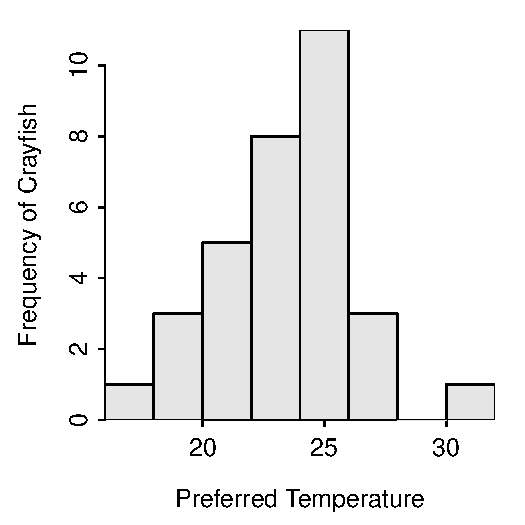
\includegraphics[width=.4\linewidth]{Figs/CrayfishTempHist-1} 

}

\caption[Histogram of crayfish temperature preferences]{Histogram of crayfish temperature preferences.}\label{fig:CrayfishTempHist}
\end{figure}


\end{knitrout}

% latex table generated in R 3.4.0 by xtable 1.8-2 package
% Sun May 21 17:06:49 2017
\begin{table}[ht]
\centering
\caption{Descriptive statistics of crayfish temperature preferences.} 
\label{tab:CrayfishTempStats}
\begin{tabular}{rrrrrrrr}
  \hline
n & mean & sd & min & Q1 & median & Q3 & max \\ 
  \hline
32.00 & 22.88 & 2.79 & 16.00 & 21.00 & 23.00 & 25.00 & 30.00 \\ 
   \hline
\end{tabular}
\end{table}


\begin{minipage}{\textwidth}
R Appendix:
\begin{knitrout}
\definecolor{shadecolor}{rgb}{0.922, 0.922, 0.922}\color{fgcolor}\begin{kframe}
\begin{verbatim}
setwd("c:/data/")
cray <- read.csv("Crayfish.csv")
str(cray)
hist(~temp,data=cray,xlab="Preferred Temperature",ylab="Frequency of Crayfish",w=2)
Summarize(~temp,data=cray,digits=2)
\end{verbatim}
\end{kframe}
\end{knitrout}
\end{minipage}

\newpage
\begin{exsection}
  \item \label{revex:quEDACP} \rhw{} Construct a proper EDA for the creatine phosphokinase data presented in Exercise \ref{revex:quEDACreatPhosph}. Make sure to defend your choice of numerical summaries. \ansref{ans:quEDACP}
  \item \label{revex:quEDADJTI} \rhw{} \hspace{12pt} The Dow Jones Travel Index tracks the cost of hotel and car-rental rates in 20 major cities. For its May 7, 1996, survey the following rates were given for the 20 cities: 152, 180, 167, 119, 115, 113, 119, 135, 140, 126, 114, 133, 205, 104, 149, 124, 127, 161, 106, and 179. Thoroughly describe the distribution of these data. [\textit{Note: You can use fewer than the ideal number of bars on your histogram because the sample size is so small in this situation.}] \ansref{ans:quEDADJTI}
  \item \label{revex:quEDAZoo2} \rhw{} The data in \href{https://raw.githubusercontent.com/droglenc/NCData/master/Zoo2.csv}{Zoo2.csv} contains the physical size (in acres) of a sample of zoos from around the United States. Perform a univariate EDA on the \var{size} variable. \ansref{ans:quEDAZoo2}
\end{exsection}






    \part{Inference Concepts}





    \part{Specific Hypothesis Tests}






    \cleardoublepage
    \phantomsection
    \addcontentsline{toc}{part}{Appendix}
    \chapter*{Appendices}
    \appendix



  \backmatter
    %BIBLIOGRAPHY ---------------------------------------------------------------------------------------------------------
\cleardoublepage                             %not sure why but this is needed so TOC entry will point to right start page
\phantomsection                              %not sure why but this is needed so TOC entry will point to right start page
\addcontentsline{toc}{part}{Bibliography}    %Add a TOC entry
\bibliography{c:/aaaWork/zGnrlLatex/DHO_Bib} %make the bibliography
 
%INDEX ----------------------------------------------------------------------------------------------------------------
% cross references for the index
\index{Alternative Hypothesis|see{Hypothesis, Alternative}}
\index{Coefficient of Determination|see{$r^{2}$}}
\index{Forward calculation|see{Normal Distribution, Finding areas}}
\index{Frequency Table|see{Table, Frequency}}
\index{Goodness-of-Fit Test|see{Chi-square}}
\index{Line!Finding best-fit|see{Regression}}
\index{Mean!Inference|see{Z-test and t-Test}}
\index{Null Hypothesis|see{Hypothesis, Null}}
\index{Percentage Table|see{Table}}
\index{Proportions Table|see{Table, Proportion}}
\index{Row Proportions Table|see{Table, Proportion}}
\index{Column Proportions Table|see{Table, Proportion}}
\index{Table Proportions Table|see{Table, Proportion}}
\index{Proportions, Inference|see{Chi-square}}
\index{Rejection Criterion|see{$\alpha$}}
\index{Reverse calculation|see{Normal Distribution, Finding values}}
\index{Simple Linear Regression|see{Regression}}
\index{SLR|see{Regression}}
\index{Standard Normal Distribution|see{Normal Distribution}}
\index{Standardization|see{Normal Distribution, Converting to Z-scale}}
\index{One-sample Z-Test|see{Z-Test}}
\index{1-sample Z-Test|see{Z-Test}}
\index{One-sample t-Test|see{t-Test}}
\index{1-sample t-Test|see{t-Test}}
\index{Two-sample t-Test|see{t-Test}}
\index{2-sample t-Test|see{t-Test}}
\index{Matched-Pairs t-Test|see{t-Test}}
\index{Two-way Table|see{Table, Frequency}}
\index{Type I Error|see{Hypothesis Testing, Errors}}
\index{Type II Error|see{Hypothesis Testing, Errors}}
\index{Variability!Natural|see{Natural Variability}}
\index{Variability!Sampling|see{Sampling Variability}}
\index{Variable!Types|see{Quantitative, Continuous, Discrete, Categorical, Nominal, or Ordinal}}
\index{Variance!Testing Equality|see{Levene's Test}}
\index{Y-intercept|see{Intercept}}
\index{Z-Distribution|see{Normal Distribution, Standard Normal}}

% code to actually add the index
\addtocontents{toc}{\setlength{\cftbeforepartskip}{0.4em}}  %decrease dist before parts in back matter portion of TOC
\cleardoublepage                          %not sure why but this is needed so TOC entry will point to right start page
\phantomsection                           %not sure why but this is needed so TOC entry will point to right start page
\addcontentsline{toc}{part}{Index}        %Add a TOC entry
\printindex                               %Make the index


\end{document}
